\documentclass[12pt, twoside]{article}
\usepackage[utf8]{inputenc}
\usepackage[english]{babel}

\usepackage{amsthm}
\usepackage{a4wide}
\usepackage{graphicx}
\usepackage{caption}
\usepackage{amssymb}
\usepackage{amsmath}
\usepackage{mathrsfs}
\usepackage{euscript}
\usepackage{graphicx}
\usepackage{subfig}
\usepackage{caption}
\usepackage{color}
\usepackage{bm}
\usepackage{tabularx}
\usepackage{adjustbox}


\usepackage[toc,page]{appendix}

\usepackage{comment}
\usepackage{rotating}

\DeclareMathOperator*{\argmax}{arg\,max}
\DeclareMathOperator*{\argmin}{arg\,min}

\newtheorem{theorem}{Theorem}
\newtheorem{lemma}[theorem]{Lemma}
\newtheorem{definition}{Definition}[section]

\numberwithin{equation}{section}

\newcommand*{\No}{No.}

\usepackage{autonum}

\begin{document}

\title{\bf Prior distribution choices for a mixture of experts \thanks{This research was supported by RFBR (project ???) and NTI (project ???).}}
\date{}
\author{}
\maketitle

\begin{center}
\bf
A. V. Grabovoy\footnote{Moscow Institute of Physics and Technology, grabovoy.av@phystech.edu},
V. V. Strijov\footnote{Moscow Institute of Physics and Technology, Dorodnicyn Computing Centre, Federal Research Center “Computer Science and Control” of the Russian Academy of Sciences, strijov@phystech.edu}
\end{center}
{\centering\begin{quote}
\textbf{Abstract:} 
The paper investigates a mixture of expert models. 
The mixture of experts is a combination of experts, local approximation model, and a gate function, which weighs these experts and forms their ensemble. 
In this work, each expert is a linear model.
The gate function is a neural network with softmax on the last layer. 
The paper analyzes various prior distributions for each expert.
The authors propose a method that takes into account the relationship between prior distributions of different experts.
The EM algorithm optimises both parameters of the local models and parameters of the gate function.
As an application problem, the paper solves a problem of shape recognition on images.
Each expert fits one circle in an image and recovers its parameters: the coordinates of the center and the radius.
The computational experiment uses synthetic and real data to test the proposed method.
The real data is a human eye image from the iris detection problem.


\smallskip
\textbf{Keywords}: mixture of Experts; bayesian model selection; prior distribution.

\smallskip
\end{quote}
}

\section{Introduction}
The paper studies the problem of mixture of experts construction.
The mixture of experts is a multimodel. The mixture of experts uses a gate function to weight predictions of each expert.
It is a combination of weighed local models to approximate a dataset.
The weighting coefficients depend on objects in the dataset.
Examples of multimodel are bagging, gradient boosting~\cite{Tianqi2016} and random forest~\cite{Ishwaran2012}. 
The paper~\cite{Yuksel2012} suggests that the contribution of each expert to the answer depends on the object from the dataset.

The main problem of multimodel construction is hight dependence of the resulted ensemble on the initial value of the parameters.
The authors propose to use the probability approach to find optimal gate function parameters and local parameters, and proposes to use various prior distributions of the parameters to improve stability of the multimodel.
The paper introduces a method, which use dependence between prior distributions to improve the multimodel quality.

\begin{figure}[h!t]\center
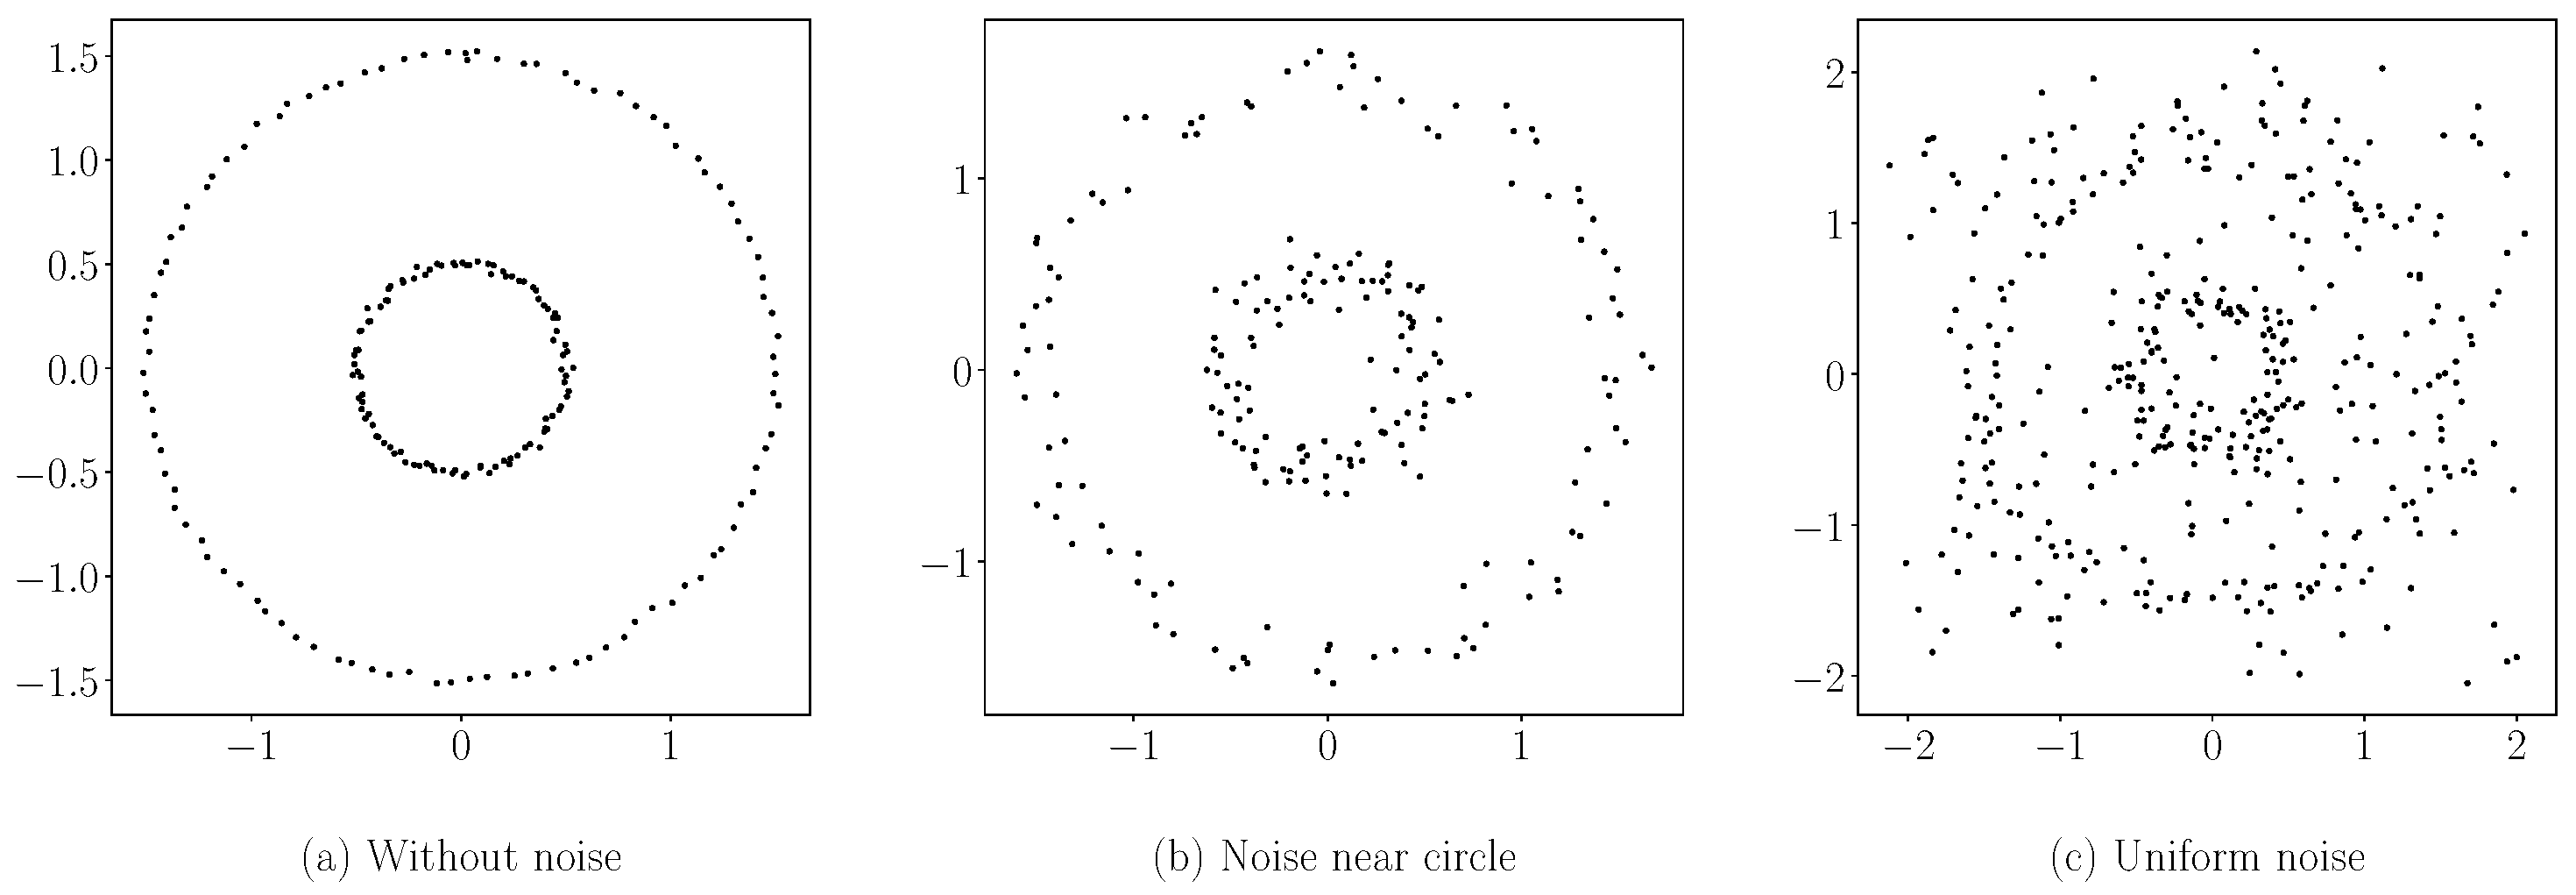
\includegraphics[width=1\textwidth]{result_eng/statment}
\caption{An example of circles with different noise levels: (a) circle without noise; (b) noisy radius circle; (c) noisy radius circle, and uniform noisy on image}
\label{example:1}
\end{figure}

As a practical example, the circles approximation on a binarized image are solved.
Examples of images are shown in fig.~\ref{example:1}.
In this paper, each expert is a linear model.
A gate function is a two-layer fully connected neural network.

\paragraph{Related work.}
Many papers on a mixture of experts are devoted to gateway function selection: softmax, the Dirichlet process~\cite{Edward2002}, neural networks~\cite{Shazeer2017} with softmax function on the last layer.
Some papers are devoted to the choice of the expert type. 
Papers~\cite{Jordan1994, Jordan1991} analyze linear models as experts.
Papers~\cite{Lima2007, Cao2003} analyze SVMs as experts.
The paper~\cite{Yuksel2012} contains an overview of various gate function and various expert types.

The method of mixture of experts has many applications.
Papers~\cite{Yumlu2003, Cheung1995, Weigend2000} use the mixture of experts in time series forecasting.
Paper~\cite{Ebrahimpour2009} uses the mixture of experts in the task of recognizing handwritten numbers.
Papers~\cite{Estabrooks2001, Mossavat2010, Peng1996, Tuerk2001}  are devoted to methods of text and speech recognition by using the mixture of experts.
Paper~\cite{Sminchisescu2007} analyzes the mixture of experts to recognize three-dimensional human movements.
Paper~\cite{Bowyer2010} is devoted to a review of the study results on the iris detection in the image.
The methods of highlighting the borders of the iris and pupil are described in papers~\cite{Matveev2010, Matveev2014}.

\section{Problem statement of circle parameters estimation}
There given binary image
\[
\label{eq:st:cr:1}
\begin{aligned}
\textbf{M} \in \{0,1\}^{m_1 \times m_2},
\end{aligned}
\]
where~$1$ is a black pixel, an image foreground, and~$0$ is a white pixel, the image background. 
An image example is shown in fig.~\ref{example:1}.
The image~$\textbf{M}$ is mapped to a set of coordinates~\mbox{$\textbf{C}=\left\{x_i, y_i\right\}_{i=1}^{N}$}. The pair of coordinates~$(x_i, y_i)$ is a black pixel in~$\textbf{M}$:
\[
\label{eq:st:cr:2}
\begin{aligned}
\textbf{C} \in  \mathbb{R}^{N \times 2},
\end{aligned}
\]
where~$N$ is the number of black pixels.

Let~$(x_0, y_0)$ be the center of the circle, and~$r$ is radius of the circle.
 The coordinates~$\left(x_i, y_i\right)\in\textbf{C}$ is a circle locus of points defined by
\[
\label{eq:st:cr:3}
\begin{aligned}
\bigr(x_i - x_0\bigr)^{2}+\bigr(y_i-y_0\bigr)^2 = r^2.
\end{aligned}
\]
Expand brackets:
\[
\label{eq:st:cr:4}
\begin{aligned}
\left(2x_0\right)\cdot x_i + \left(2y_0\right)\cdot y_i+\left(r^2-x_0^2-y_0^2\right)\cdot1 = x_{i}^2 + y_{i}^2.
\end{aligned}
\]
Rewrite equation~\eqref{eq:st:cr:4} to set the linear regressions problem for all points in the dataset:
\[
\label{eq:st:cr:5}
\begin{aligned}
\hat{\textbf{w}} = \arg\min_{\textbf{w}\in \mathbf{R}^{n}}||\textbf{X}\textbf{w} - \textbf{y}||,  \quad \textbf{X} = \left[\textbf{C}, \textbf{1}\right], \quad \textbf{y} = \left[x_1^2+y_1^2, x_2^2+y_2^2, \cdots, x_N^2+y_N^2\right]^{\mathsf{T}}.
\end{aligned}
\]
The parameters~$\hat{\textbf{w}} = \left[w_1, w_2, w_3\right]^{\mathsf{T}}$ reconstruct the circle parameters~$x_0, y_0, r$:
\[
\label{eq:st:cr:6}
\begin{aligned}
x_0 = \frac{w_1}{2}, \quad y_0 = \frac{w_2}{2}, \quad r = \sqrt[]{w_3+x_{0}^{2}+y_{0}^{2}}.
\end{aligned}
\]
The solution of problem~\eqref{eq:st:cr:5} reconstructs the circle parameters only if the number of circles in an image is equal to one.
The authors propose to use the multimodel for the image, which consists of several circles.
The multimodel is an ensemble of the linear models.
Each linear model approximates only one circle in the image.
In this paper, multimodel is a mixture of experts.

\section{Problem statement of building a mixture of experts}
Generalize one-circle approximation~\eqref{eq:st:cr:5} problem to the case of several circles.
Each circle is a local model.
The data for this case is
\[
\label{eq:st:1}
\begin{aligned}
\textbf{X} \in \mathbb{R}^{N \times n}, \quad \textbf{y}\in \mathbb{R}^{N}
\end{aligned}
\]
where~$N$ is the sample size and~$n$ is the number of features. In this paper,~$n$ is equal to~$3$.

\begin{definition}
\label{def:1}
A model~$\mathbf{g}$ is a local model on dataset~$\textbf{X}$ if~$\mathbf{g}$ approximates some no-empty subset~$\textbf{X}'\subset\textbf{X}$.
\end{definition}

\begin{definition}
\label{def:2}
Call the multimodel~$\mathbf{f}$ a mixture of experts
\[
\label{eq:st:2}
\begin{aligned}
\mathbf{f} = \sum_{k=1}^{K}\pi_{k}\mathbf{g}_k\bigr(\mathbf{w}_k\bigr), \qquad \pi_{k}\bigr(\mathbf{x}, \mathbf{V}\bigr):\mathbb{R}^{n\times \left|\mathbf{V}\right|} \to [0, 1], \qquad \sum_{k=1}^{K}\pi_{k}\bigr(\mathbf{x}, \mathbf{V}\bigr) = 1,
\end{aligned}
\]
where~$\mathbf{g}_k$ is a local model,~$\pi_k$ is a gate function, vector~$\mathbf{w}_k$ is some parameters of the local model and~$\mathbf{V}$ is some parameters of the gate function.
\end{definition}

This paper asserts the local model be linear model. The gate function is the two--layer fully connected neural network
\[
\label{eq:st:3}
\begin{aligned}
\mathbf{g}_k\bigr(\textbf{x}\bigr) = \textbf{w}_k^{\mathsf{T}}\textbf{x}, \quad
\bm{\pi}\bigr(\mathbf{x}, \mathbf{V}\bigr) = \text{softmax}\bigr(\mathbf{V}_{1}^{\mathsf{T}}\bm{\sigma}\bigr(\mathbf{V}_2^{\mathsf{T}}\mathbf{x}\bigr)\bigr),
\end{aligned}
\]
where~$\mathbf{V} = \bigr\{\mathbf{V}_1, \mathbf{V}_2\bigr\}$ is a set of the gate function parameters.

The paper proposes to use a probabilistic approach to describe a mixture of experts. Let~$\textbf{y}$ be a random variable with density function~$p\bigr(\textbf{y}|\textbf{X}\bigr)$. Let density~$p\bigr(\textbf{y}|\textbf{X}, \textbf{f}\bigr)$ approximate truth density~$p\bigr(\textbf{y}|\textbf{X}\bigr)$:
\[
\label{eq:st:new:1}
\begin{aligned}
p\bigr(\textbf{y}|\textbf{X}, \textbf{f}\bigr) = \prod_{i=1}^{N}\left(\sum_{k=1}^{K}\pi_kp_{k}\bigr(y_{i}|\textbf{g}_{k}\bigr(\mathbf{x}_{i}\bigr)\bigr)\right),
\end{aligned}
\]
where~$\textbf{f}$ is the mixture of experts and~$\textbf{g}_k, \bm{\pi}$ are defined by~\eqref{eq:st:3}.

%Combining~\eqref{eq:st:2} and~\eqref{eq:st:3}, obtain the likelihood solution:
Suppose that~$\textbf{w}_k$ is the random variable with density function~$p^{k}\bigr(\mathbf{w}_k\bigr)$, and get joint probability distribution of the target and the parameters:
\[
\label{eq:st:4}
\begin{aligned}
p\bigr(\mathbf{y}, \mathbf{W}|\mathbf{X}, \mathbf{V}\bigr) = \prod_{k=1}^{K}p^{k}\bigr(\mathbf{w}_k\bigr)\prod_{i=1}^{N}\left(\sum_{k=1}^{K}\pi_{k}p_{k}\bigr(y_i|\mathbf{w}_k, \mathbf{x}_i\bigr)\right),
\end{aligned}
\]
where~$\mathbf{W} = \bigr\{\mathbf{w}_1, \mathbf{w}_2, \cdots, \mathbf{w}_K\bigr\}.$
The optimal parameters is delivered by the evidence maximisation:
\[
\label{eq:st:5}
\begin{aligned}
\hat{\mathbf{V}} = \arg\max_{\mathbf{V}} p\bigr(\mathbf{y}|\mathbf{X}, \mathbf{V}\bigr).
\end{aligned}
\]

\section{Probabilistic statement of mixture of expert}
To build the mixture of experts~(\ref{eq:st:2}, ~\ref{eq:st:4}), set the following probabilistic statement for the dataset~\eqref{eq:st:1}:

\begin{enumerate}
	\item[1)] the likelihood~$p_{k}\bigr(y_{i}|\mathbf{w}_{k}, \mathbf{x}_{i}\bigr) = \mathcal{N}\bigr(y_{i}|\mathbf{w}_{k}^{\mathsf{T}}\mathbf{x}_{i}, \beta^{-1}\bigr),$ where parameter~$\beta$ is the noise level,
	\item[2)] the prior distribution for the parameters~$p^{k}\bigr(\mathbf{w}_{k}\bigr) = \mathcal{N}\bigr(\mathbf{w}_{k}|\mathbf{w}^{0}_{k}, \mathbf{A}_{k}\bigr),$ where~$\mathbf{w}^{0}_{k}$ is a vector of size~$n\times1$ and~$\mathbf{A}_{k}$ is a covariance matrix,
	\item[3)] the prior regularisation~$p\bigr(\bm{\varepsilon}_{k,k'}|\bm{\Xi}\bigr) = \mathcal{N}\bigr(\bm{\varepsilon}_{k,k'}|\mathbf{0},  \bm{\Xi}\bigr),$ where~$\bm{\Xi}$ is a covariance matrix and~$\bm{\varepsilon}_{k,k'} = \mathbf{w}_{k}^{0}-\mathbf{w}_{k'}^{0}.$
\end{enumerate}
The assumption 2) is the prior distribution for the parameters~$\textbf{w}_k$. It sets some restrictions to the model. For example, if~$\textbf{w}_k^{0}$ is [0,0,1], then the~$k$-th local model fits with the most probability a circle with parameters~$x_0=0, y_0=0, r=1$.

The assumption 3) is a prior regularisation. It sets restrictions on the prior distribution parameters. For example, if~$\text{diag}\bigr(\bm{\Xi}\bigr)=[0.001, 0.001, 1]$, then the centers of different circles, which corresponds to different local models are equal.

Combining assumptions~$1), 2), 3)$ and equation~\eqref{eq:st:4}, obtain the new likelihood:
\[
\label{eq:em:1}
\begin{aligned}
p\bigr(\mathbf{y}, \mathbf{W}|\mathbf{X}, \mathbf{V}, \textbf{A}, \textbf{W}^{0}, \bm{\Xi}, \beta\bigr) = &\prod_{i=1}^{N}\left(\sum_{k=1}^{K}\pi_{k}\mathcal{N}\bigr(y_{i}|\mathbf{w}_{k}^{\mathsf{T}}\mathbf{x}_{i}, \beta^{-1}\bigr)\right)\cdot\\
&\cdot\prod_{k=1}^{K}\mathcal{N}\bigr(\mathbf{w}_{k}|\mathbf{w}^{0}_{k}, \mathbf{A}_{k}\bigr)\cdot\prod_{k,k'=1}^{K}\mathcal{N}\bigr(\bm{\varepsilon}_{k,k'}|\mathbf{0},  \bm{\Xi}\bigr),
\end{aligned}
\]
 where~$\mathbf{A} = \left\{\mathbf{A}_1, \cdots, \mathbf{A}_K\right\}.$
 
Introduce a binary matrix~$\mathbf{Z}$. Its element~$z_{ik}$ is equal to~$1$ if and only if the~$i$-th object corresponds to the~$k$-th local model.
Using the binary matrix~$\mathbf{Z}$ in~\eqref{eq:em:1} take logarithm and obtain
\[
\label{eq:em:2}
\begin{aligned}
\log p\bigr(\mathbf{y}, \mathbf{Z}, \mathbf{W}&|\mathbf{X}, \mathbf{V}, \textbf{A}, \textbf{W}^{0},  \bm{\Xi}, \beta\bigr) =\\
&= \sum_{i=1}^{N}\sum_{k=1}^{K}z_{ik}\left[\log\pi_k\bigr(\textbf{x}_i, \textbf{V}\bigr) - \frac{\beta}{2}\left(y_{i} - \textbf{w}_{k}^{\mathsf{T}}\textbf{x}_{i}\right)^{2} + \frac{1}{2}\log\frac{\beta}{2\pi}\right] +\\
&+ \sum_{k=1}^{K}\left[-\frac{1}{2}\left(\textbf{w}_{k} - \textbf{w}_{k}^{0}\right)^{\mathsf{T}}\textbf{A}_{k}^{-1}\left(\textbf{w}_{k} - \textbf{w}_{k}^{0}\right) + \frac{1}{2}\log\det\textbf{A}^{-1}_{k} - \frac{n}{2}\log2\pi\right]+\\
&+ \sum_{k=1}^{K}\sum_{k'=1}^{K}\left[-\frac{1}{2}\left(\textbf{w}_{k}^{0}-\textbf{w}_{k'}^{0}\right)^{\mathsf{T}}\bm{\Xi}^{-1}\left(\textbf{w}_{k}^{0}-\textbf{w}_{k'}^{0}\right) +\frac{1}{2}\log\det \bm{\Xi} -\frac{n}{2}\log{2\pi}\right].
\end{aligned}
\]
Set the new optimisation problem to optimise the evidence function. The function is obtained by integrating equation~\eqref{eq:em:2} over parameters~$\textbf{W}, \textbf{Z}$:
\[
\label{eq:em:3}
\begin{aligned}
\mathbf{V}, \mathbf{W}^0, \textbf{A},  \beta = \arg\max_{\mathbf{V}, \mathbf{W}^0, \textbf{A}, \beta} \int_{\textbf{W}, \textbf{Z}}\log p\bigr(\mathbf{y}, \textbf{Z}, \textbf{W}|\mathbf{X}, \mathbf{V}, \textbf{A}, \textbf{W}^{0}, \bm{\Xi}, \beta\bigr)d\textbf{W}d\textbf{Z}.
\end{aligned}
\]
\section{EM--algorithm as a solver of optimisation problem}
Let~$q\bigr(\textbf{W}, \textbf{Z}\bigr)$ be some density distribution of parameters~$\textbf{W}, \textbf{Z}$. Rewrite the evidence:
\[
\label{eq:em:new:1}
\begin{aligned}
\log p\bigr(\mathbf{y}|\mathbf{X}, \mathbf{V}, \textbf{A}, \textbf{W}^{0}, \bm{\Xi}, \beta\bigr) &= \int_{\textbf{W}, \textbf{Z}} q\bigr(\textbf{W}, \textbf{Z}\bigr) \log p\bigr(\mathbf{y}|\mathbf{X}, \mathbf{V}, \textbf{A}, \textbf{W}^{0}, \bm{\Xi}, \beta\bigr)d\textbf{W}d\textbf{Z} =\\
&= \int_{\textbf{W}, \textbf{Z}} q\bigr(\textbf{W}, \textbf{Z}\bigr)\log \frac{p\bigr(\mathbf{y}, \textbf{W}, \textbf{Z}|\mathbf{X}, \mathbf{V}, \textbf{A}, \textbf{W}^{0}, \bm{\Xi}, \beta\bigr)}{p\bigr(\textbf{W}, \textbf{Z}|\mathbf{y}, \mathbf{X}, \mathbf{V}, \textbf{A}, \textbf{W}^{0}, \bm{\Xi}, \beta\bigr)}d\textbf{W}d\textbf{Z}=\\
&= \int_{\textbf{W}, \textbf{Z}} q\bigr(\textbf{W}, \textbf{Z}\bigr)\log \frac{p\bigr(\mathbf{y}, \textbf{W}, \textbf{Z}|\mathbf{X}, \mathbf{V}, \textbf{A}, \textbf{W}^{0}, \bm{\Xi}, \beta\bigr)q\bigr(\textbf{W}, \textbf{Z}\bigr)}{p\bigr(\textbf{W}, \textbf{Z}|\mathbf{y}, \mathbf{X}, \mathbf{V}, \textbf{A}, \textbf{W}^{0}, \bm{\Xi}, \beta\bigr)q\bigr(\textbf{W}, \textbf{Z}\bigr)}d\textbf{W}d\textbf{Z}=\\
&= \int_{\textbf{W}, \textbf{Z}} q\bigr(\textbf{W}, \textbf{Z}\bigr)\frac{p\bigr(\mathbf{y}, \textbf{W}, \textbf{Z}|\mathbf{X}, \mathbf{V}, \textbf{A}, \textbf{W}^{0}, \bm{\Xi}, \beta\bigr)}{q\bigr(\textbf{W}, \textbf{Z}\bigr)}d\textbf{W}d\textbf{Z}+\\
&+\int_{\textbf{W}, \textbf{Z}} q\bigr(\textbf{W}, \textbf{Z}\bigr)\frac{q\bigr(\textbf{W}, \textbf{Z}\bigr)}{p\bigr(\textbf{W}, \textbf{Z}|\mathbf{y}, \mathbf{X}, \mathbf{V}, \textbf{A}, \textbf{W}^{0}, \bm{\Xi}, \beta\bigr)}d\textbf{W}d\textbf{Z}=\\
&=\mathcal{L}\bigr(q, \textbf{V}, \textbf{W}^{0}, \textbf{A}, \beta\bigr)+\mathsf{D}_{KL}\left(q\bigr(\textbf{W}, \textbf{Z}\bigr)||p\bigr(\textbf{W}, \textbf{Z}|\mathbf{y}, \mathbf{X}, \mathbf{V}, \textbf{A}, \textbf{W}^{0}, \bm{\Xi}, \beta\bigr)\right)
\end{aligned}
\]
Using~\eqref{eq:em:new:1}, we get lower bound of evidence:
\[
\label{eq:em:new:2}
\begin{aligned}
\log p\bigr(\mathbf{y}|\mathbf{X}, \mathbf{V}, \textbf{A}, \textbf{W}^{0}, \bm{\Xi}, \beta\bigr)\geq \mathcal{L}\bigr(q, \textbf{V}, \textbf{W}^{0}, \textbf{A}, \beta\bigr),
\end{aligned}
\]
where~$\mathcal{L}\bigr(q, \textbf{V}, \textbf{W}^{0}, \textbf{A}, \beta\bigr)$ is called lower bound of evidence.

Use the expectation-maximization~\cite{Dempster1977, bishop2006} algorithm to find the solution to optimisation problem~\eqref{eq:em:3}. The EM-algorithm instead of~$\log p\bigr(\mathbf{y}|\mathbf{X}, \mathbf{V}, \textbf{A}, \textbf{W}^{0}, \bm{\Xi}, \beta\bigr)$ optimizes the lower bound~$\mathcal{L}\left(q, \textbf{V}, \textbf{W}^{0}, \textbf{A}, \beta\right)$.


\paragraph{E-step.} E-step solves the optimisation problem:
\[
\label{eq:em:new:3}
\begin{aligned}
\mathcal{L}\bigr(q, \textbf{V}, \textbf{W}^{0}, \textbf{A}, \beta\bigr) \to \max_{q\bigr(\textbf{W}, \textbf{Z}\bigr)},
\end{aligned}
\]
where~$\textbf{V}, \textbf{W}^{0}, \textbf{A}, \beta$ are fixed.

Let the joint distribution~$q\bigr(\mathbf{Z}, \mathbf{W}\bigr)$ satisfies the assumption of independence~$q\bigr(\mathbf{Z}, \mathbf{W}\bigr) = q\bigr(\mathbf{Z}\bigr)q\bigr(\mathbf{W}\bigr)$~\cite{bishop2006}. 
The symbol~$\propto$ means that both sides are equal to up to an additive constant.
First, find the distribution~$q\bigr(\textbf{Z}\bigr)$:
\[
\label{eq:em:4}
\begin{aligned}
\log q\bigr(\textbf{Z}\bigr) &= \mathsf{E}_{q/\textbf{Z}} \log p\bigr(\mathbf{y}, \mathbf{Z}, \mathbf{W}|\mathbf{X}, \mathbf{V}, \textbf{A}, \textbf{W}^{0}, \bm{\Xi}, \beta\bigr)  \propto\\
&\propto \sum_{i+1}^{N}\sum_{k=1}^{K}z_{ik}\left[\log\pi_{k}\bigr(\textbf{x}_{i}, \textbf{V}\bigr) - \frac{\beta}{2}\left(y_{i}^{2} -\textbf{x}_{i}^{\mathsf{T}}\mathsf{E}\textbf{w}_{k} + \textbf{x}_{i}^{\mathsf{T}}\mathsf{E}\textbf{w}_{k}\textbf{w}_{k}^{\mathsf{T}}\textbf{x}_{i}\right) + \frac{1}{2}\log\frac{\beta}{2\pi}\right]\\
p\bigr(z_{ik} = 1\bigr) &= \frac{\exp\bigr(\log\pi_{k}\bigr(\textbf{x}_{i}, \textbf{V}\bigr) - \frac{\beta}{2}\left(\textbf{x}_{i}^{\mathsf{T}}\mathsf{E}\textbf{w}_{k}\textbf{w}_{k}^{\mathsf{T}}\textbf{x}_{i} - \textbf{x}_{i}^{\mathsf{T}}\mathsf{E}\textbf{w}_{k}\right)\bigr)}{\sum_{k'=1}^{K}\exp\bigr(\log\pi_{k'}\bigr(\textbf{x}_{i}, \textbf{V}\bigr) - \frac{\beta}{2}\left(\textbf{x}_{i}^{\mathsf{T}}\mathsf{E}\textbf{w}_{k'}\textbf{w}_{k'}^{\mathsf{T}}\textbf{x}_{i} - \textbf{x}_{i}^{\mathsf{T}}\mathsf{E}\textbf{w}_{k'}\right)\bigr)}.
\end{aligned}
\]
Using~\eqref{eq:em:4}, we get that distribution~$q\bigr(z_{ik}\bigr)$ is the Bernoulli distribution with probability~$z_{ik}$ from equation~\eqref{eq:em:4}.
Second, find the distribution~$q\bigr(\textbf{W}\bigr)$:
\[
\label{eq:em:5}
\begin{aligned}
\log q\bigr(\textbf{W}\bigr) &= \mathsf{E}_{q/\textbf{W}}\log p\bigr(\mathbf{y}, \mathbf{Z}, \mathbf{W}|\mathbf{X}, \mathbf{V}, \textbf{A}, \textbf{W}^{0}, \bm{\Xi}, \beta\bigr) \propto\\
&\propto \sum_{i=1}^{N}\sum_{k=1}^{K}\mathsf{E}z_{ik}\left[\log\pi_{k}\bigr(\textbf{x}_{i, \textbf{V}}\bigr) - \frac{\beta}{2}\left(y_{i} - \textbf{w}_{k}^{\mathsf{T}}\textbf{x}_{i}\right)^{2} + \frac{1}{2}\log\frac{\beta}{2\pi}\right] + \\
&+ \sum_{k=1}^{K}\left[-\frac{1}{2}\left(\textbf{w}_{k} - \textbf{w}_{k}^{0}\right)^{\mathsf{T}}\textbf{A}_{k}^{-1}\left(\textbf{w}_{k} - \textbf{w}_{k}^{0}\right) + \frac{1}{2}\log\det\textbf{A}^{-1}_{k} - \frac{n}{2}\log2\pi\right] \\
&\propto \sum_{k=1}^{K}\left[\textbf{w}_{k}^{\mathsf{T}}\left(\textbf{A}_{k}^{-1}\textbf{w}_{k}^{0}+\beta\sum_{i=1}^{N}\textbf{x}_{i}y_{i}\mathsf{E}z_{ik}\right)-\frac{1}{2}\textbf{w}_{k}^{\mathsf{T}}\left(\textbf{A}_{k}^{-1}+\beta\sum_{i=1}^{N}\textbf{x}_{i}\textbf{x}_{i}^{\mathsf{T}}\right)\textbf{w}_{k}\right].
\end{aligned}
\]
Using~\eqref{eq:em:5}, we get that distribution~$q\bigr(\mathbf{w}_{k}\bigr)$ is the normal distribution with mean~$\mathbf{m}_{k}$ and covariance matrix~$\mathbf{B}_k$:
\[
\label{eq:em:6}
\begin{aligned}
\mathbf{m}_{k} = \mathbf{B}_{k}\left(\mathbf{A}_{k}^{-1}\mathbf{w}_{k}^{0}+\beta\sum_{i=1}^{N}\mathbf{x}_{i}y_{i}\mathsf{E}z_{ik}\right), \qquad \mathbf{B}_{k} = \left(\mathbf{A}_{k}^{-1}+\beta\sum_{i=1}^{N}\mathbf{x}_{i}\mathbf{x}_{i}^{\mathsf{T}}\mathsf{E}z_{ik}\right)^{-1}.
\end{aligned}
\]

\paragraph{M-step.} M-step solves the optimisation problem:
\[
\label{eq:em:new:3}
\begin{aligned}
\mathcal{L}\bigr(q, \textbf{V}, \textbf{W}^{0}, \textbf{A}, \beta\bigr) \to \max_{\textbf{V}, \textbf{W}^{0}, \textbf{A}, \beta},
\end{aligned}
\]
where~$q\bigr(\textbf{W}, \textbf{Z}\bigr)$ are fixed density function.
The distribution~$q\bigr(\mathbf{Z}, \mathbf{W}\bigr)$ is fixed, while the lower bound~$\mathcal{L}\bigr(\textbf{V}, \textbf{W}^{0}, \textbf{A}, \beta\bigr)$  is maximized with respect to the parameters~$\mathbf{V}, \mathbf{W}^0, \textbf{A},  \beta$:
\[
\label{eq:em:7}
\begin{aligned}
\mathcal{L}\bigr(\textbf{V}, \textbf{W}^{0}, \textbf{A}, \beta\bigr) &= \mathsf{E}_{q}\log p\bigr(\mathbf{y}, \mathbf{Z}, \mathbf{W}|\mathbf{X}, \mathbf{V}, \textbf{A}, \textbf{W}^{0}, \bm{\Xi}, \beta\bigr) =  \\
&= \sum_{i=1}^{N}\sum_{k=1}^{K}\mathsf{E}z_{ik}\left[\log\pi_k\bigr(\textbf{x}_i, \textbf{V}\bigr) - \frac{\beta}{2}\mathsf{E}\left(y_{i} - \textbf{w}_{k}^{\mathsf{T}}\textbf{x}_{i}\right)^{2} + \frac{1}{2}\log\frac{\beta}{2\pi}\right] +\\
&+ \sum_{k=1}^{K}\left[-\frac{1}{2}\mathsf{E}\left(\textbf{w}_{k} - \textbf{w}_{k}^{0}\right)^{\mathsf{T}}\textbf{A}_{k}^{-1}\left(\textbf{w}_{k} - \textbf{w}_{k}^{0}\right) + \frac{1}{2}\log\det\textbf{A}^{-1}_{k} - \frac{n}{2}\log2\pi\right] +\\
&+ \sum_{k=1}^{K}\sum_{k'=1}^{K}\left[-\frac{1}{2}\left(\textbf{w}_{k}^{0}-\textbf{w}_{k'}^{0}\right)^{\mathsf{T}}\bm{\Xi}^{-1}\left(\textbf{w}_{k}^{0}-\textbf{w}_{k'}^{0}\right) +\frac{1}{2}\log\det\bm{\Xi} -\frac{n}{2}\log{2\pi}\right].
\end{aligned}
\]
First, to find the optimal parameters~$\textbf{V}$, use the gradient optimisation algorithm. It convergences to some local maximum.
Second, using~\eqref{eq:em:7}, we get optimal value for~$\textbf{A}_{k}$
\[
\label{eq:em:9}
\begin{aligned}
\frac{\partial \mathcal{L}\bigr(\textbf{V}, \textbf{W}^{0}, \textbf{A}, \beta\bigr)}{\partial \textbf{A}^{-1}_k} &=  \frac{1}{2}\textbf{A}_{k} - \frac{1}{2}\mathsf{E}\left(\textbf{w}_{k} - \textbf{w}_{k}^{0}\right)\left(\textbf{w}_{k} - \textbf{w}_{k}^{0}\right)^{\mathsf{T}} = 0,\\
\textbf{A}_{k} &= \mathsf{E}\textbf{w}_{k}\textbf{w}_{k}^{\mathsf{T}} - \textbf{w}_{k}^{0}\mathsf{E}\textbf{w}_{k}^{\mathsf{T}} - \mathsf{E}\textbf{w}_{k}\textbf{w}_{k}^{0\mathsf{T}} + \textbf{w}_{k}^{0}\textbf{w}_{k}^{0\mathsf{T}}.
\end{aligned}
\]
Similarly, we get optimal value for~$\beta$ and for~$\textbf{w}_{k}^{0}$
\[
\label{eq:em:10}
\begin{aligned}
\frac{\partial \mathcal{L}\bigr(\textbf{V}, \textbf{W}^{0}, \textbf{A}, \beta\bigr)}{\partial \beta} &= \sum_{k=1}^{K}\sum_{i=1}^{N}\left(\frac{1}{\beta}\mathsf{E}z_{ik}-\frac{1}{2}\mathsf{E}z_{ik}\left[y_{i}^{2}-2y_{i}\textbf{x}_{i}^{\mathsf{T}}\mathsf{E}\textbf{w}_{k}+\textbf{x}_{i}^{\mathsf{T}}\textbf{w}_{k}\textbf{w}_{k}^{\mathsf{T}}\textbf{x}_{i}\right]\right) = 0,\\
\frac{1}{\beta}&=\frac{1}{N}\sum_{i=1}^{N}\sum_{k=1}^{K}\left[y_{i}^{2}-2y_{i}\textbf{x}_{i}^{\mathsf{T}}\mathsf{E}\textbf{w}_{k} + \textbf{x}_{i}^{\mathsf{T}}\mathsf{E}\textbf{w}_{k}\textbf{w}_{k}^{\mathsf{T}}\textbf{x}_{i}\right]\mathsf{E}z_{ik}.
\end{aligned}
\]
\[
\label{eq:em:11}
\begin{aligned}
\frac{\partial \mathcal{L}\bigr(\textbf{V}, \textbf{W}^{0}, \textbf{A}, \beta\bigr)}{\partial \mathbf{w}_k^0} &= \mathbf{A}_k^{-1}\left(\mathsf{E}\mathbf{w}_k - \mathbf{w}_{k}^{0}\right) + \bm{\Xi}\sum_{k'=1}^{K}\bigr[\mathbf{w}_{k'}^{0} -\mathbf{w}_{k}^{0}\bigr] = 0,\\
\textbf{w}_{k}^{0} &=\left[\textbf{A}_{k}^{-1}+\left(K-1\right)\bm{\Xi}\right]^{-1}\left(\textbf{A}^{-1}_{k}\mathsf{E}\textbf{w}_{k}+\bm{\Xi}\sum_{k'=1,~k'\not=k}^{K}\textbf{w}_{k'}^{0}\right).
\end{aligned}
\]
Formulas~(\ref{eq:em:4}--\ref{eq:em:11}) define an iterative procedure, which convergence to some local maximum of the optimisation problem~\eqref{eq:em:3}.

\section{Computational experiment}
The computational experiment analyzes quality of various multimodels for circle approximation.
The experiment analyzes next multimodels: multimodel~$\textbf{f}_1$ without prior distribution for the parameters, multimodel~$\textbf{f}_2$ with prior distribution~\eqref{eq:ce:1} for the parameters and multimodel~$\textbf{f}_3$ with prior regularisation.
The approximation quality of model~$\textbf{f}_i$ is
\[
\label{eq:ce:ex:0:1}
\begin{aligned}
\mathcal{S}_{\textbf{f}_i} = \sum_{k=1}^{K}\bigr(x^{k}_{0}-x^{k}_{\text{pr}}\bigr)^2+\bigr(y^{k}_{0}-y^{k}_{\text{pr}}\bigr)^2+\bigr(r^{k}-r^{k}_{\text{pr}}\bigr)^2,
\end{aligned}
\]
where~$x^{k}_0, y^{k}_0, r^{k}$ are the true center and radius for $k$-th circle,~$x^{k}_{\text{pr}}, y^{k}_{\text{pr}}, r^{k}_{\text{pr}}$ are the predicted center and radius for $k$-th circle.

To compare models with various prior distribution, use the log-likelihood without any priors~\eqref{eq:st:new:1}.
The prior distribution for the parameters in the experiment is
\[
\label{eq:ce:1}
\begin{aligned}
p^{1}\bigr(\textbf{w}_1\bigr)\sim\mathcal{N}\bigr(\textbf{w}^{0}_{1}, \textbf{I}\bigr), \quad p^{2}\bigr(\textbf{w}_2\bigr)\sim\mathcal{N}\bigr(\textbf{w}^{0}_{2}, \textbf{I}\bigr),
\end{aligned}
\]
where~$\textbf{w}^{0}_1 = [0, 0, 0.1],\ \textbf{w}^{0}_2 = [0, 0, 2]$.

\paragraph{Synthetic data with various types of noise in the image.}
\begin{figure}[h!t]\center
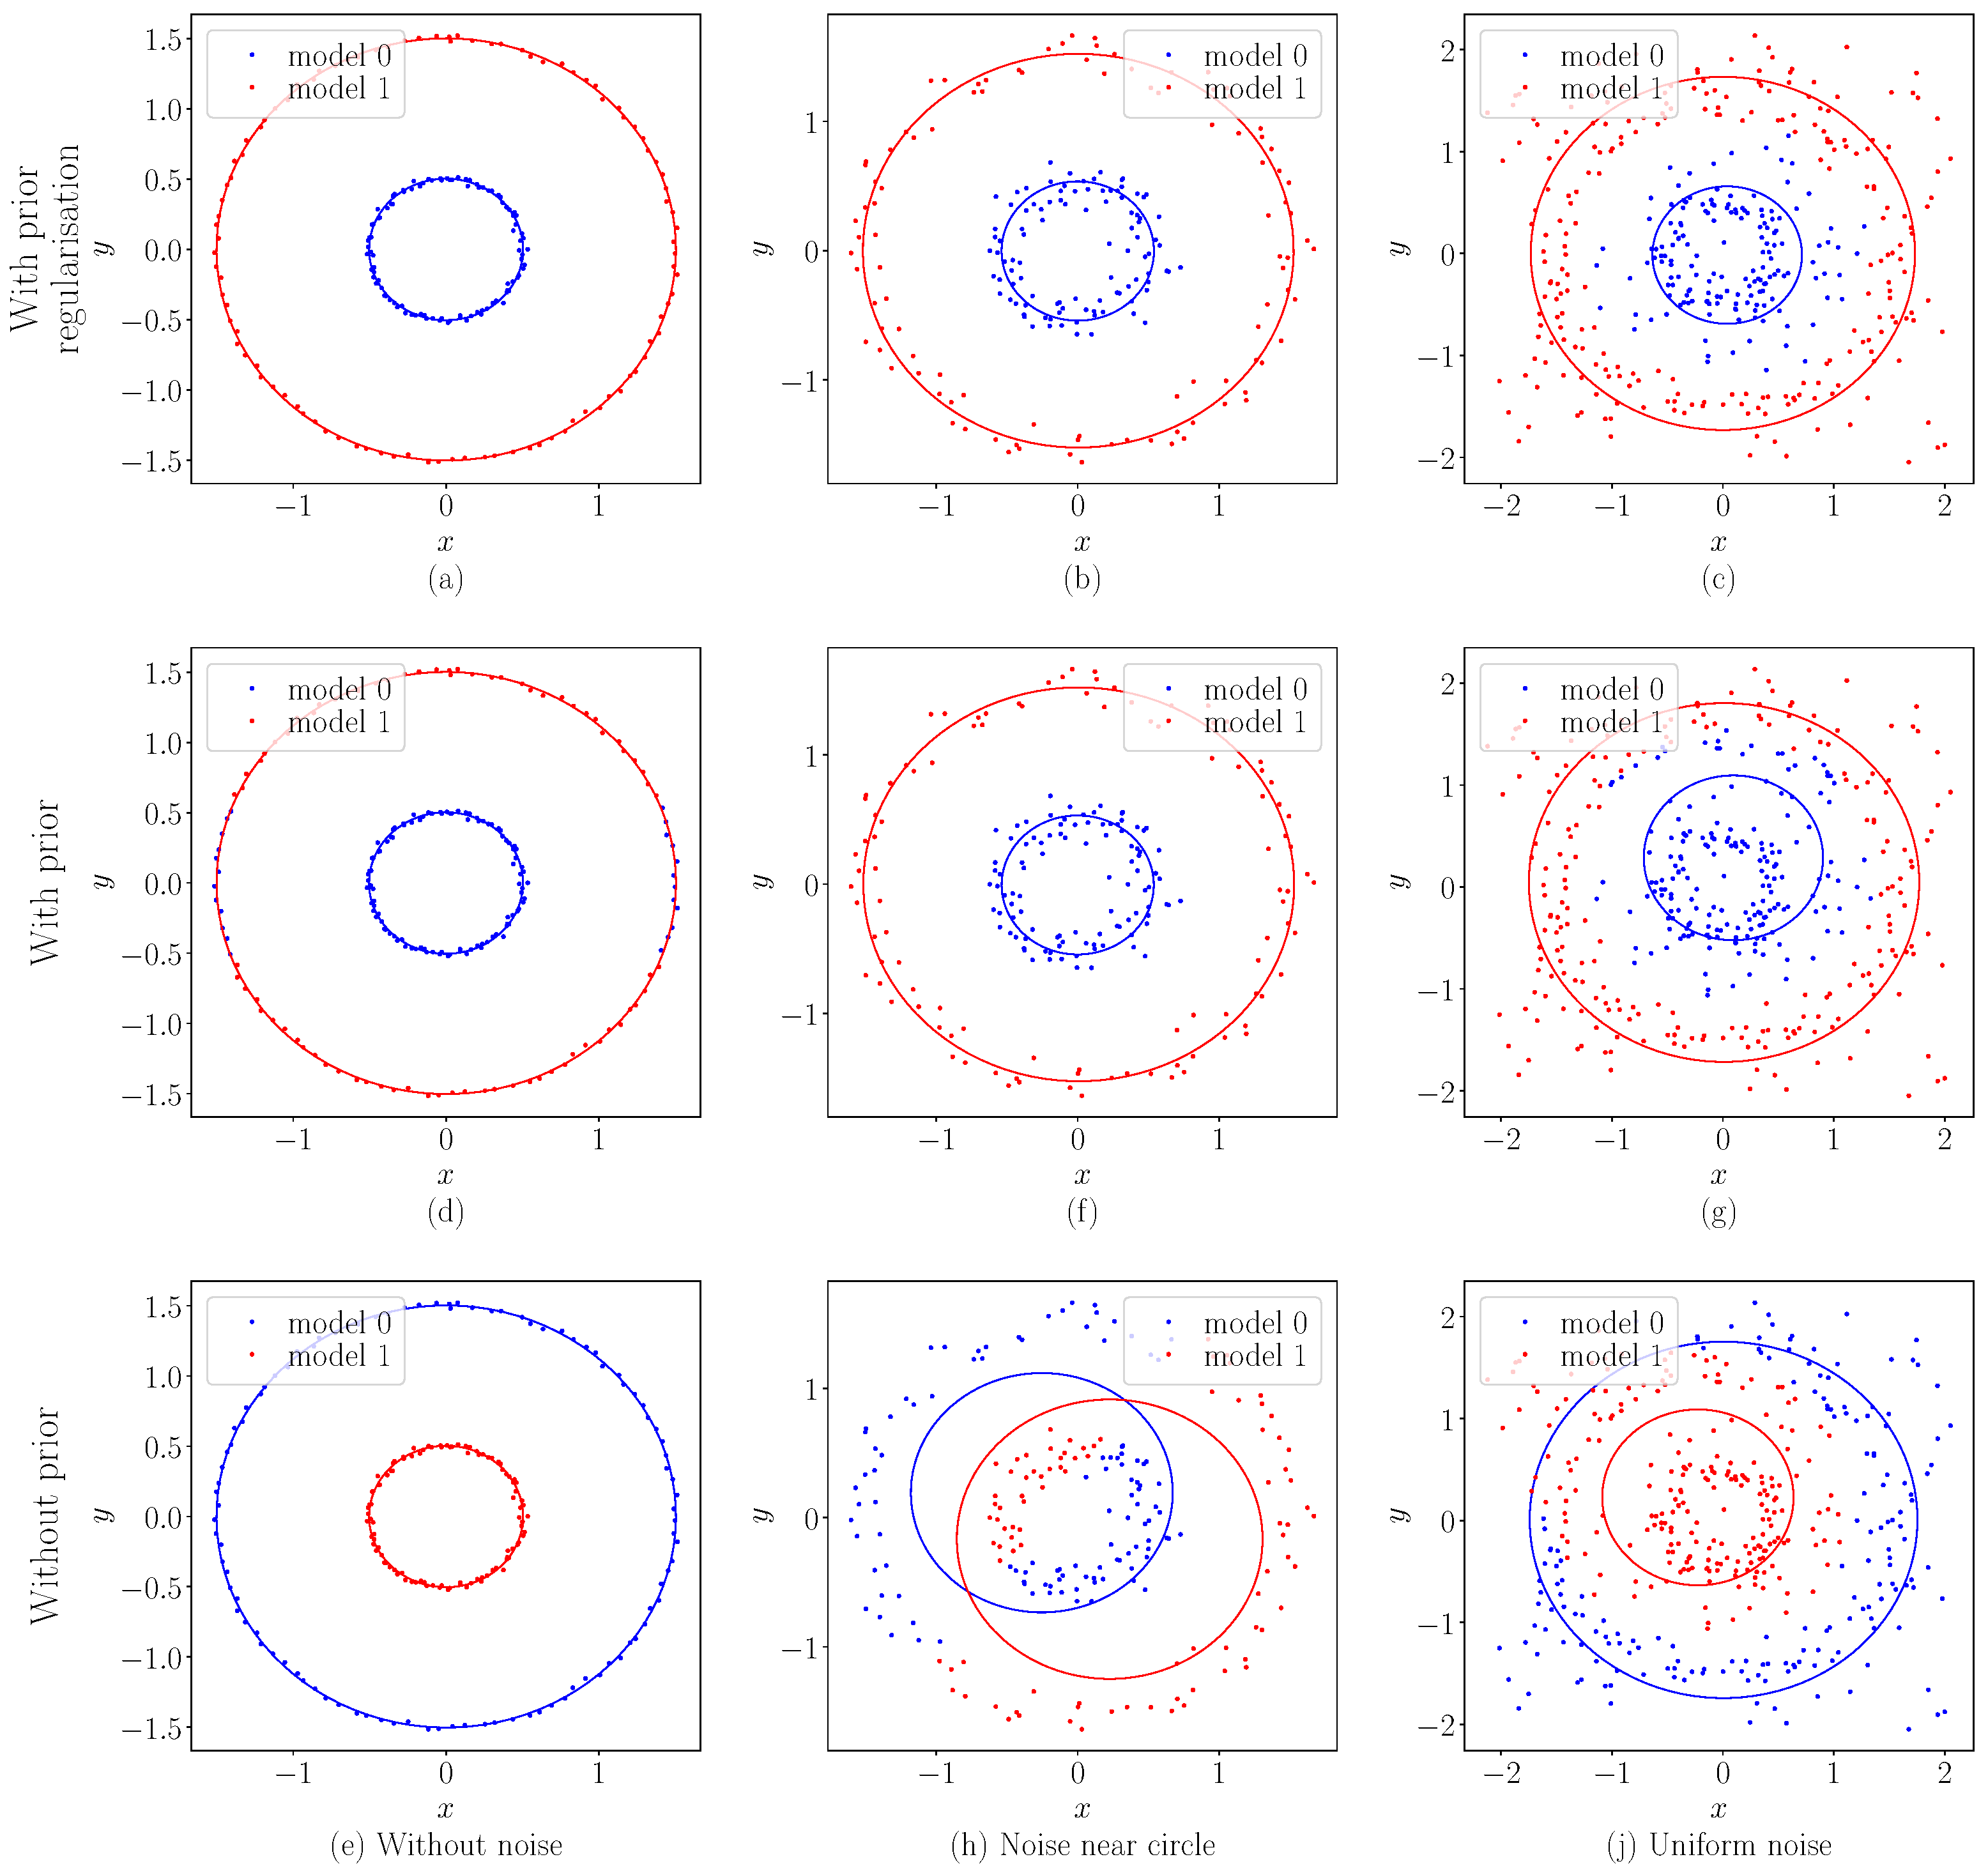
\includegraphics[width=1\textwidth]{result_eng/experiment_synthetic}
\caption{The multimodel dependes on different prior distribution and dependes on different noise levels: (a)--(c) multimodel with prior regularization; (d)--(g) multimodel with simple prior; (e)--(j) multimodel without any priors.}
\label{experiment:1}
\end{figure}
The computational experiment compares quality of mixture of experts~$\textbf{f}_1, \textbf{f}_2, \textbf{f}_3$ on a synthetic dataset.
The synthetic data were generated as two concentric circles with different noise levels.
Synthetic~1 is the image without any noises, Synthetic~2 is the image with a noise radius and the Synthetic~3 is an image with uniform noise.
The fig.~\ref{experiment:1} shows results of multimodels~$\textbf{f}_1, \textbf{f}_2, \textbf{f}_3$.
All multimodels run 50 iterations of the EM-algorithm.
Multimodels~$\textbf{f}_2, \textbf{f}_3$ approximate circles better than multimodel~$\textbf{f}_1$. Tab.~\ref{tb:ce:1} shows the approximation quality~\eqref{eq:ce:ex:0:1} for all multimodels.

\begin{table}[h!t]
\begin{center}
\caption{The approximation quality~\eqref{eq:ce:ex:0:1} for all multimodels}
\label{tb:ce:1}
\begin{tabular}{|c|c|c|c|}
\hline
	Dataset & $\mathcal{S}_{\textbf{f}_1}$ & $\mathcal{S}_{\textbf{f}_2} $& $\mathcal{S}_{\textbf{f}_3} $\\
	\hline
	\multicolumn{1}{|l|}{Synthetic~1}
	& $10^{-5}$& $10^{-5}$& $10^{-5}$\\
	\hline
	\multicolumn{1}{|l|}{Synthetic~2}
	& $0.6$& $10^{-3}$& $10^{-3}$\\
	\hline
	\multicolumn{1}{|l|}{Synthetic~3}
	& $0.6$& $10^{-3}$& $10^{-3}$\\
\hline
\end{tabular}
\end{center}
\end{table}

\paragraph{Analysis of convergence on synthetic data.}
\begin{figure}[h!t]\center
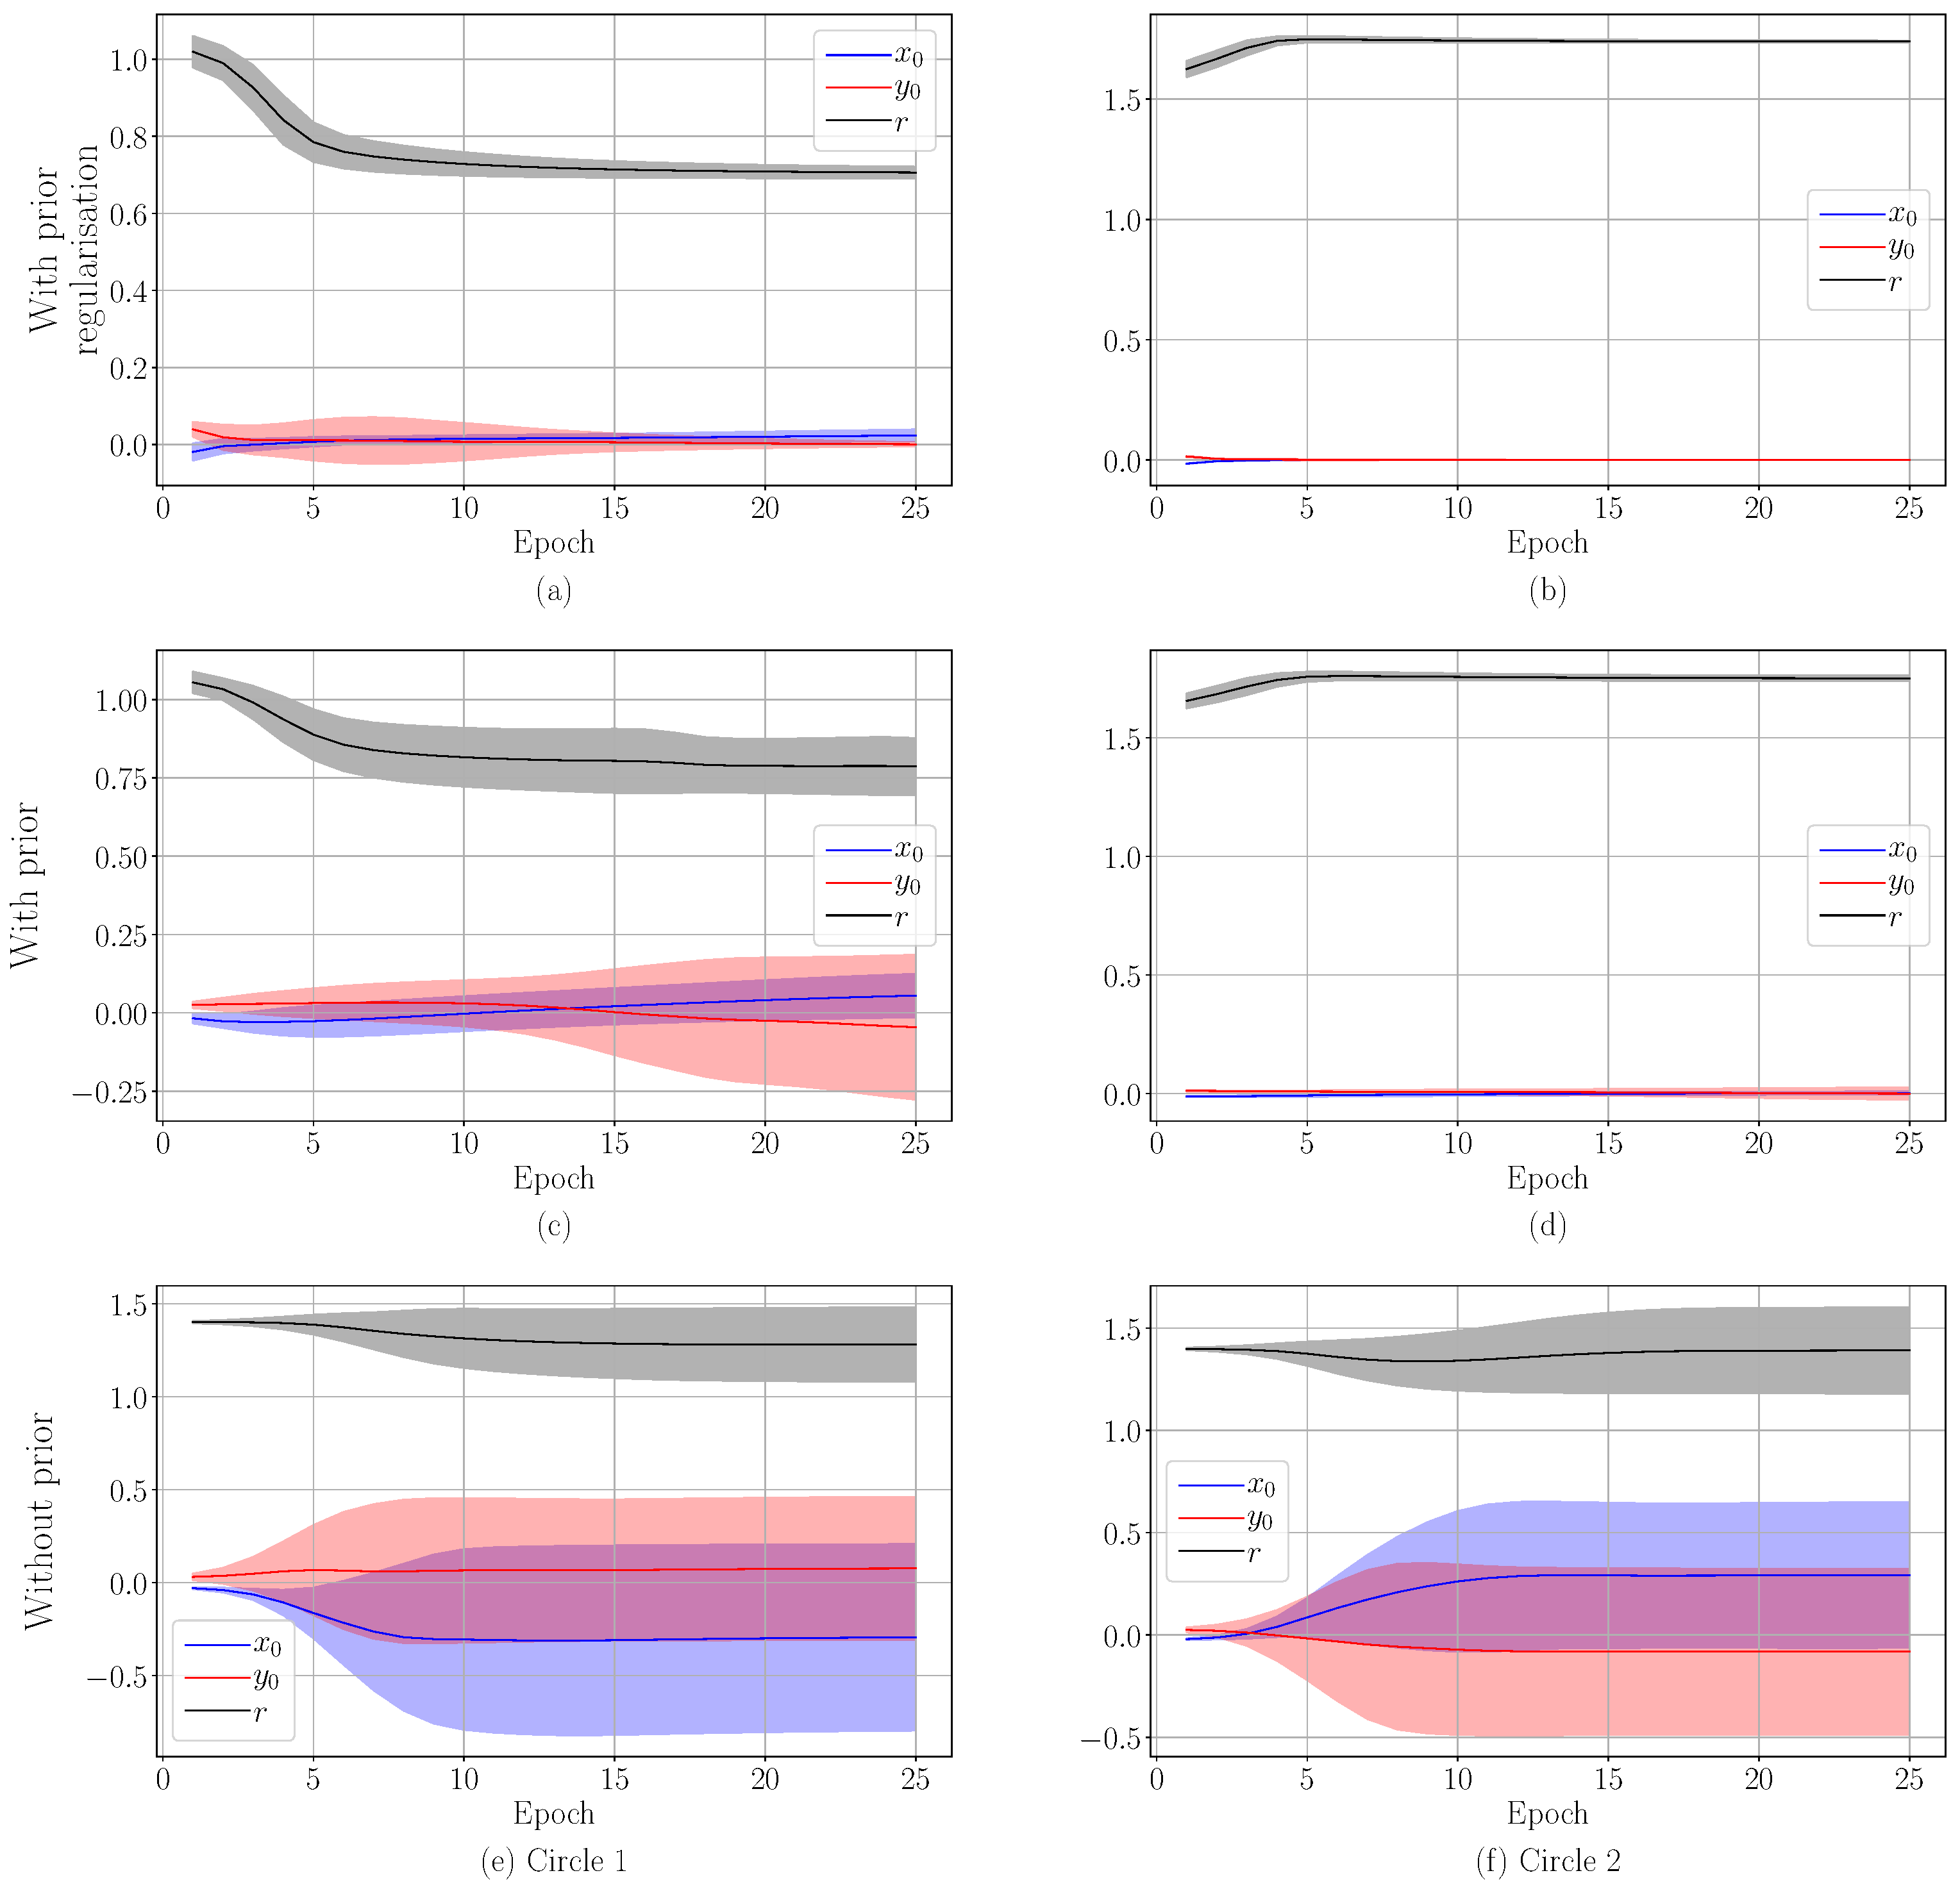
\includegraphics[width=1\textwidth]{result_eng/experiment_synthetic_param_progress}
\caption{The dependence of center and radius on the iteration number: (a)--(b) multimodel with prior regularization; (e)--(d) multimodel with simple prior; (e)--(f) multimodel without any priors.}
\label{experiment:st:2:1}
\end{figure}

\begin{figure}[h!t]\center
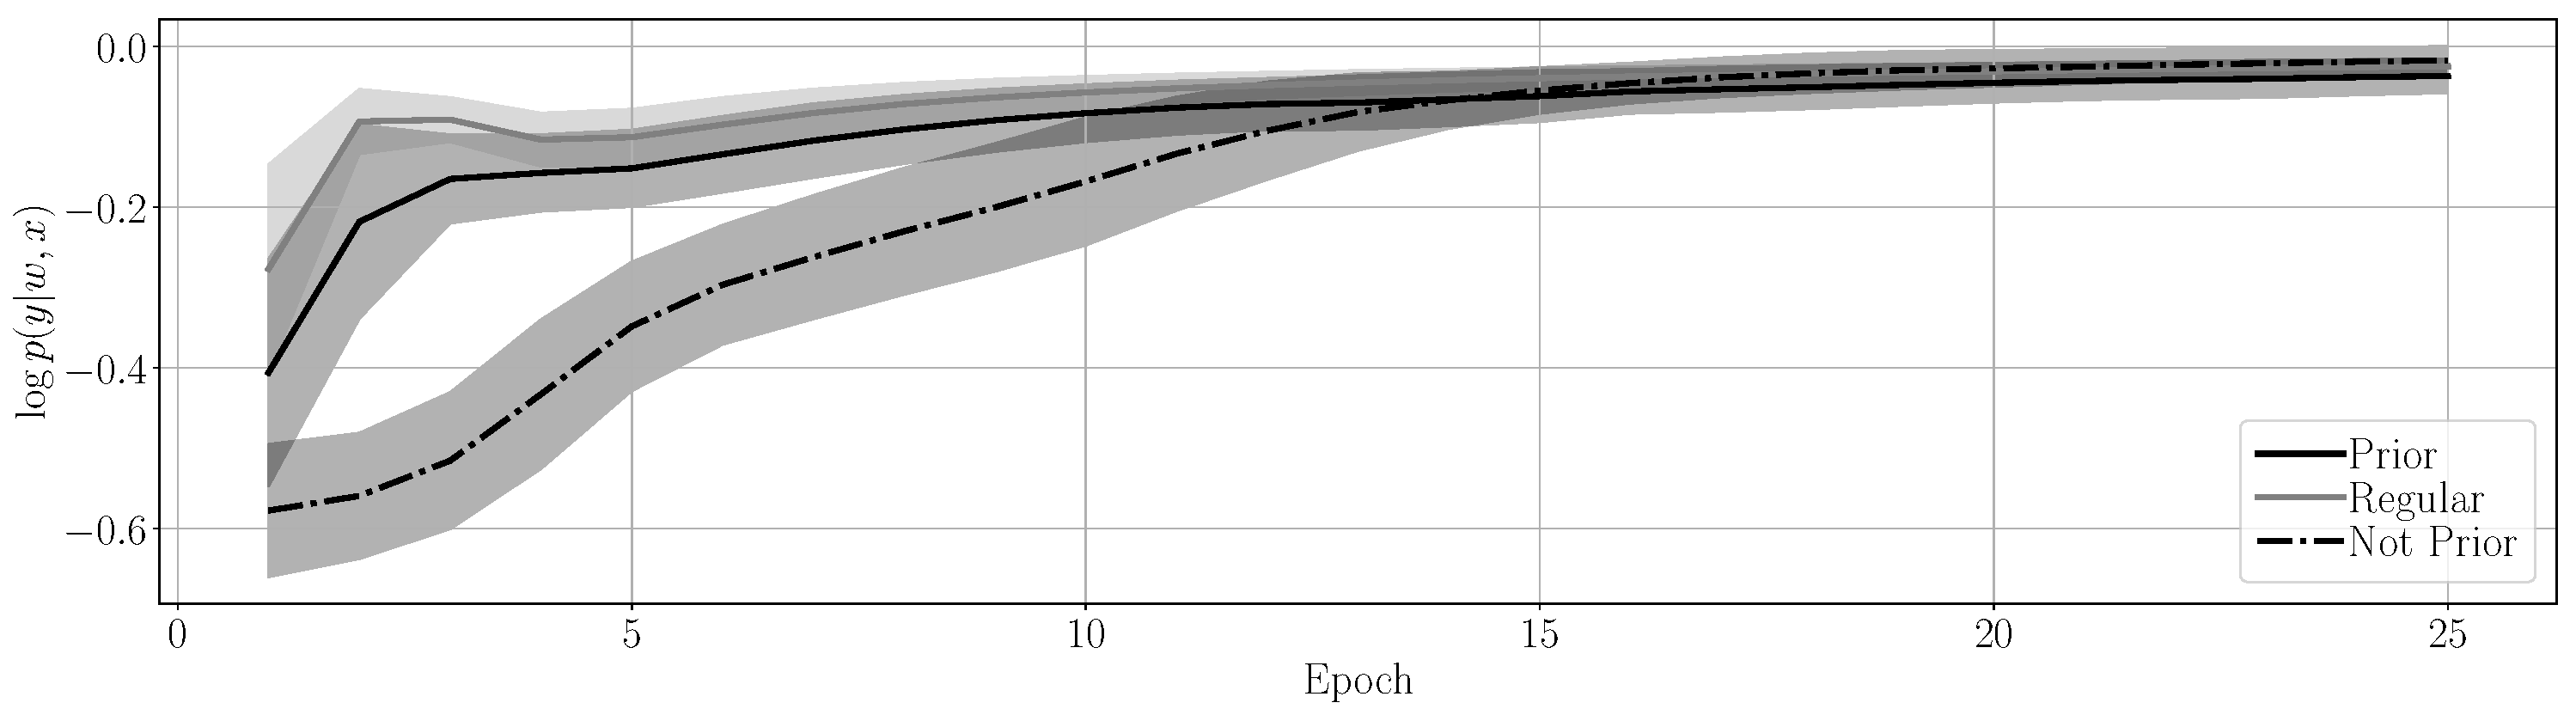
\includegraphics[width=1\textwidth]{result_eng/experiment_synt_likelihood_progress}
\caption{The dependence of log-likelihood~\eqref{eq:st:new:1} on the iteration number.}
\label{experiment:st:2:2}
\end{figure}

\begin{figure}[h!t]\center
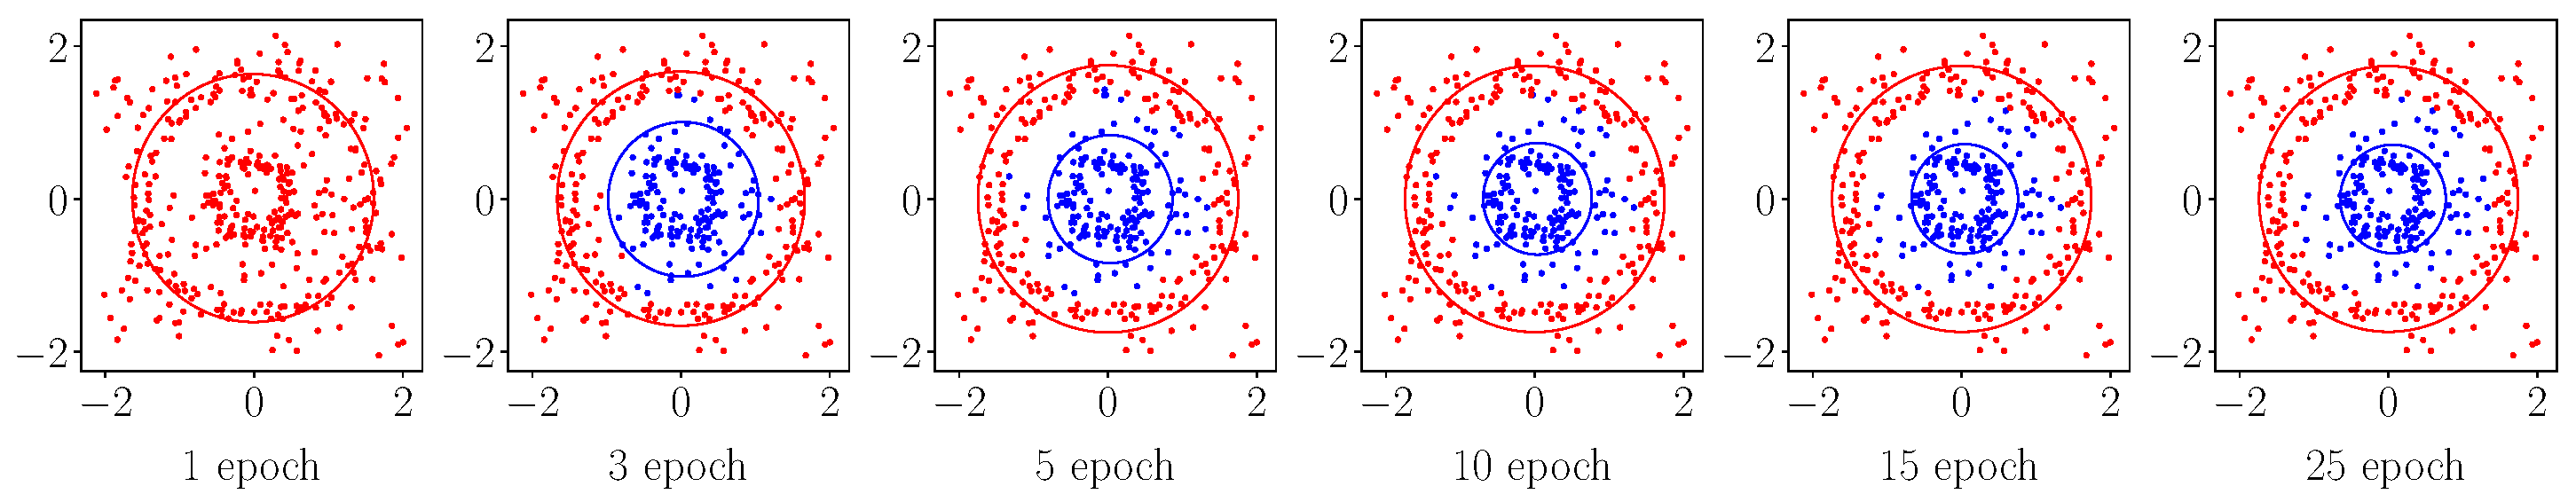
\includegraphics[width=1\textwidth]{result_eng/experiment_synt_regular_progress}
\caption{Visualization of convergence for the multimodel with prior regularisation.}
\label{experiment:st:2:3}
\end{figure}

\begin{figure}[h!t]\center
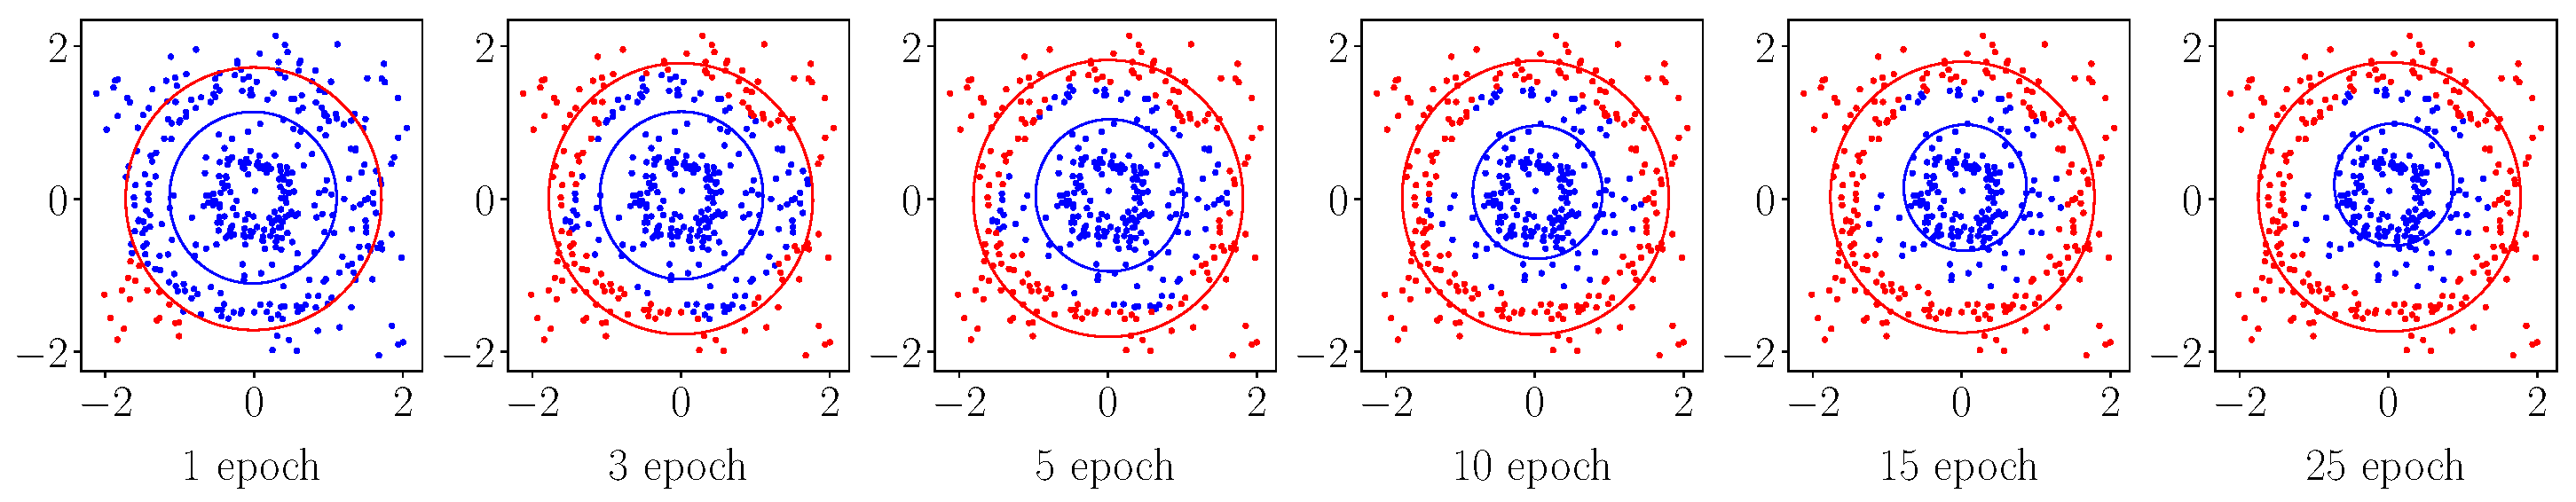
\includegraphics[width=1\textwidth]{result_eng/experiment_synt_prior_progress}
\caption{Visualization of convergence for the multimodel with simple prior.}
\label{experiment:st:2:4}
\end{figure}

\begin{figure}[h!t]\center
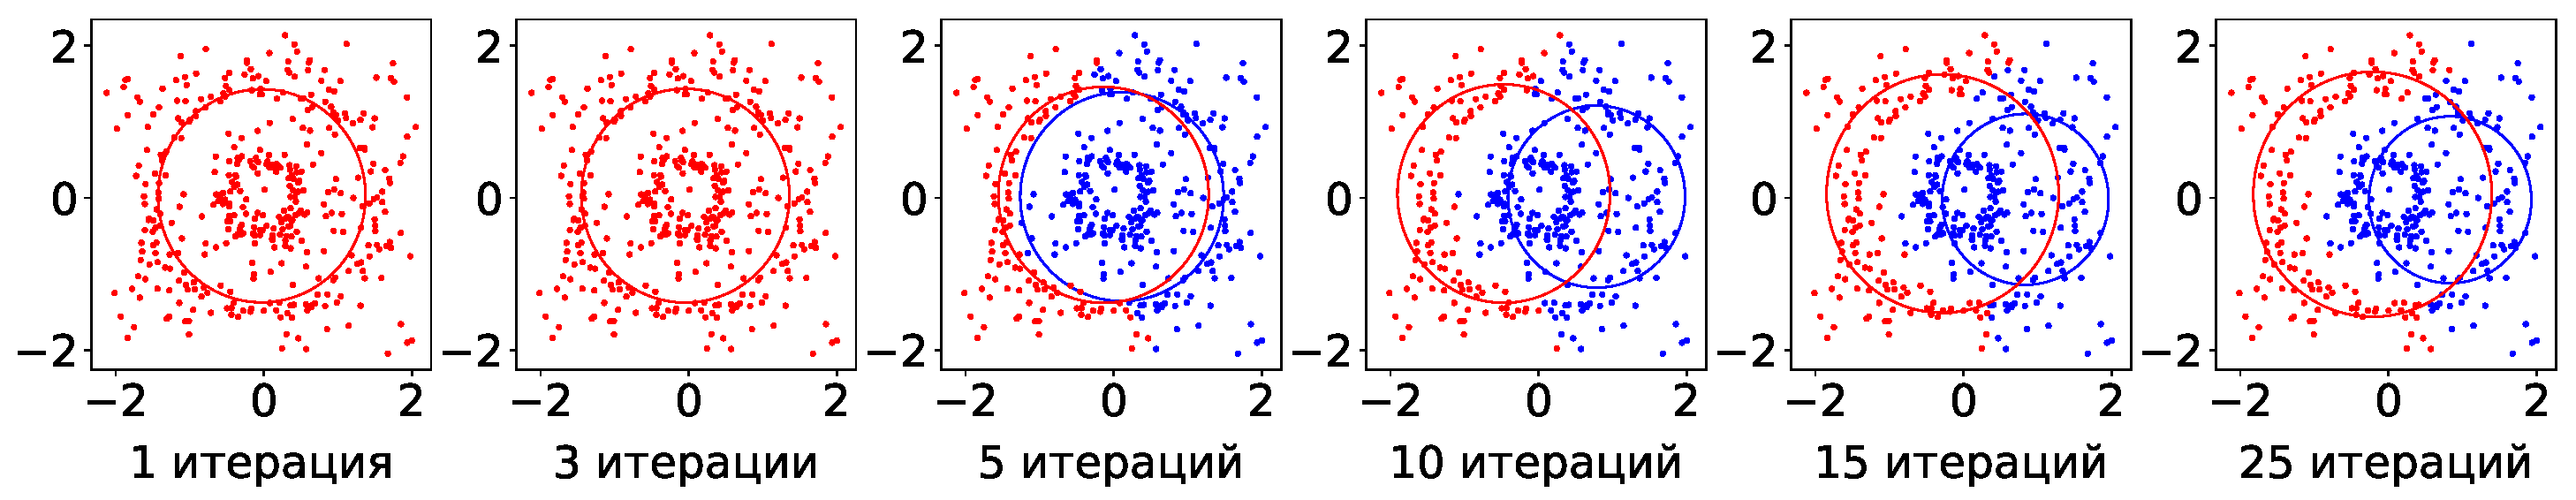
\includegraphics[width=1\textwidth]{result_eng/experiment_synt_not_prior_progress}
\caption{Visualization of convergence for the multimodel without any priors.}
\label{experiment:st:2:5}
\end{figure}
The experiment analyzes multimodels~$\textbf{f}_1, \textbf{f}_2, \textbf{f}_3$ during the EM-algorithm convergence.
The multimodels were analysed on the synthetic dataset~Synthetic~3.

Fig.~\ref{experiment:st:2:1} shows the dependence of the radius and center on the EM-algorithm iteration number.
The multimodel~$\textbf{f}_2$ with prior distribution for the parameters approximates circles better than multimodel~$\textbf{f}_1$ without any priors.
The multimodel~$\textbf{f}_3$ with prior regularisation approximates circles more stable than multimodel~$\textbf{f}_2$.

Fig.~\ref{experiment:st:2:2} shows the dependence of log-likelihood~\eqref{eq:st:new:1} on the EM-algorithm iteration number.
The log-likelihood of multimodels~$\textbf{f}_2, \textbf{f}_3$ is growing faster than multimodel~$\textbf{f}_1$.  After the $20$-th iteration all three multimodels have the same log-likelihood.

Fig.~\ref{experiment:st:2:3}-\ref{experiment:st:2:5} show learning process for multimodels~$\textbf{f}_1, \textbf{f}_2, \textbf{f}_3$.
Fig.~\ref{experiment:st:2:5} shows multimodel~$\textbf{f}_1$, which does not approximate circles correctly.
Fig.~\ref{experiment:st:2:3}-\ref{experiment:st:2:4} show multimodels~$\textbf{f}_2, \textbf{f}_3$, which approximate circles correctly.

The experiment shows that multimodels~$\textbf{f}_2, \textbf{f}_3$ with prior distribution for the parameters approximate circles better than multimodel~$\textbf{f}_1$ without any priors.


\paragraph{Multimodels analysis depending on the noise level.} 
\begin{figure}[h!t]\center
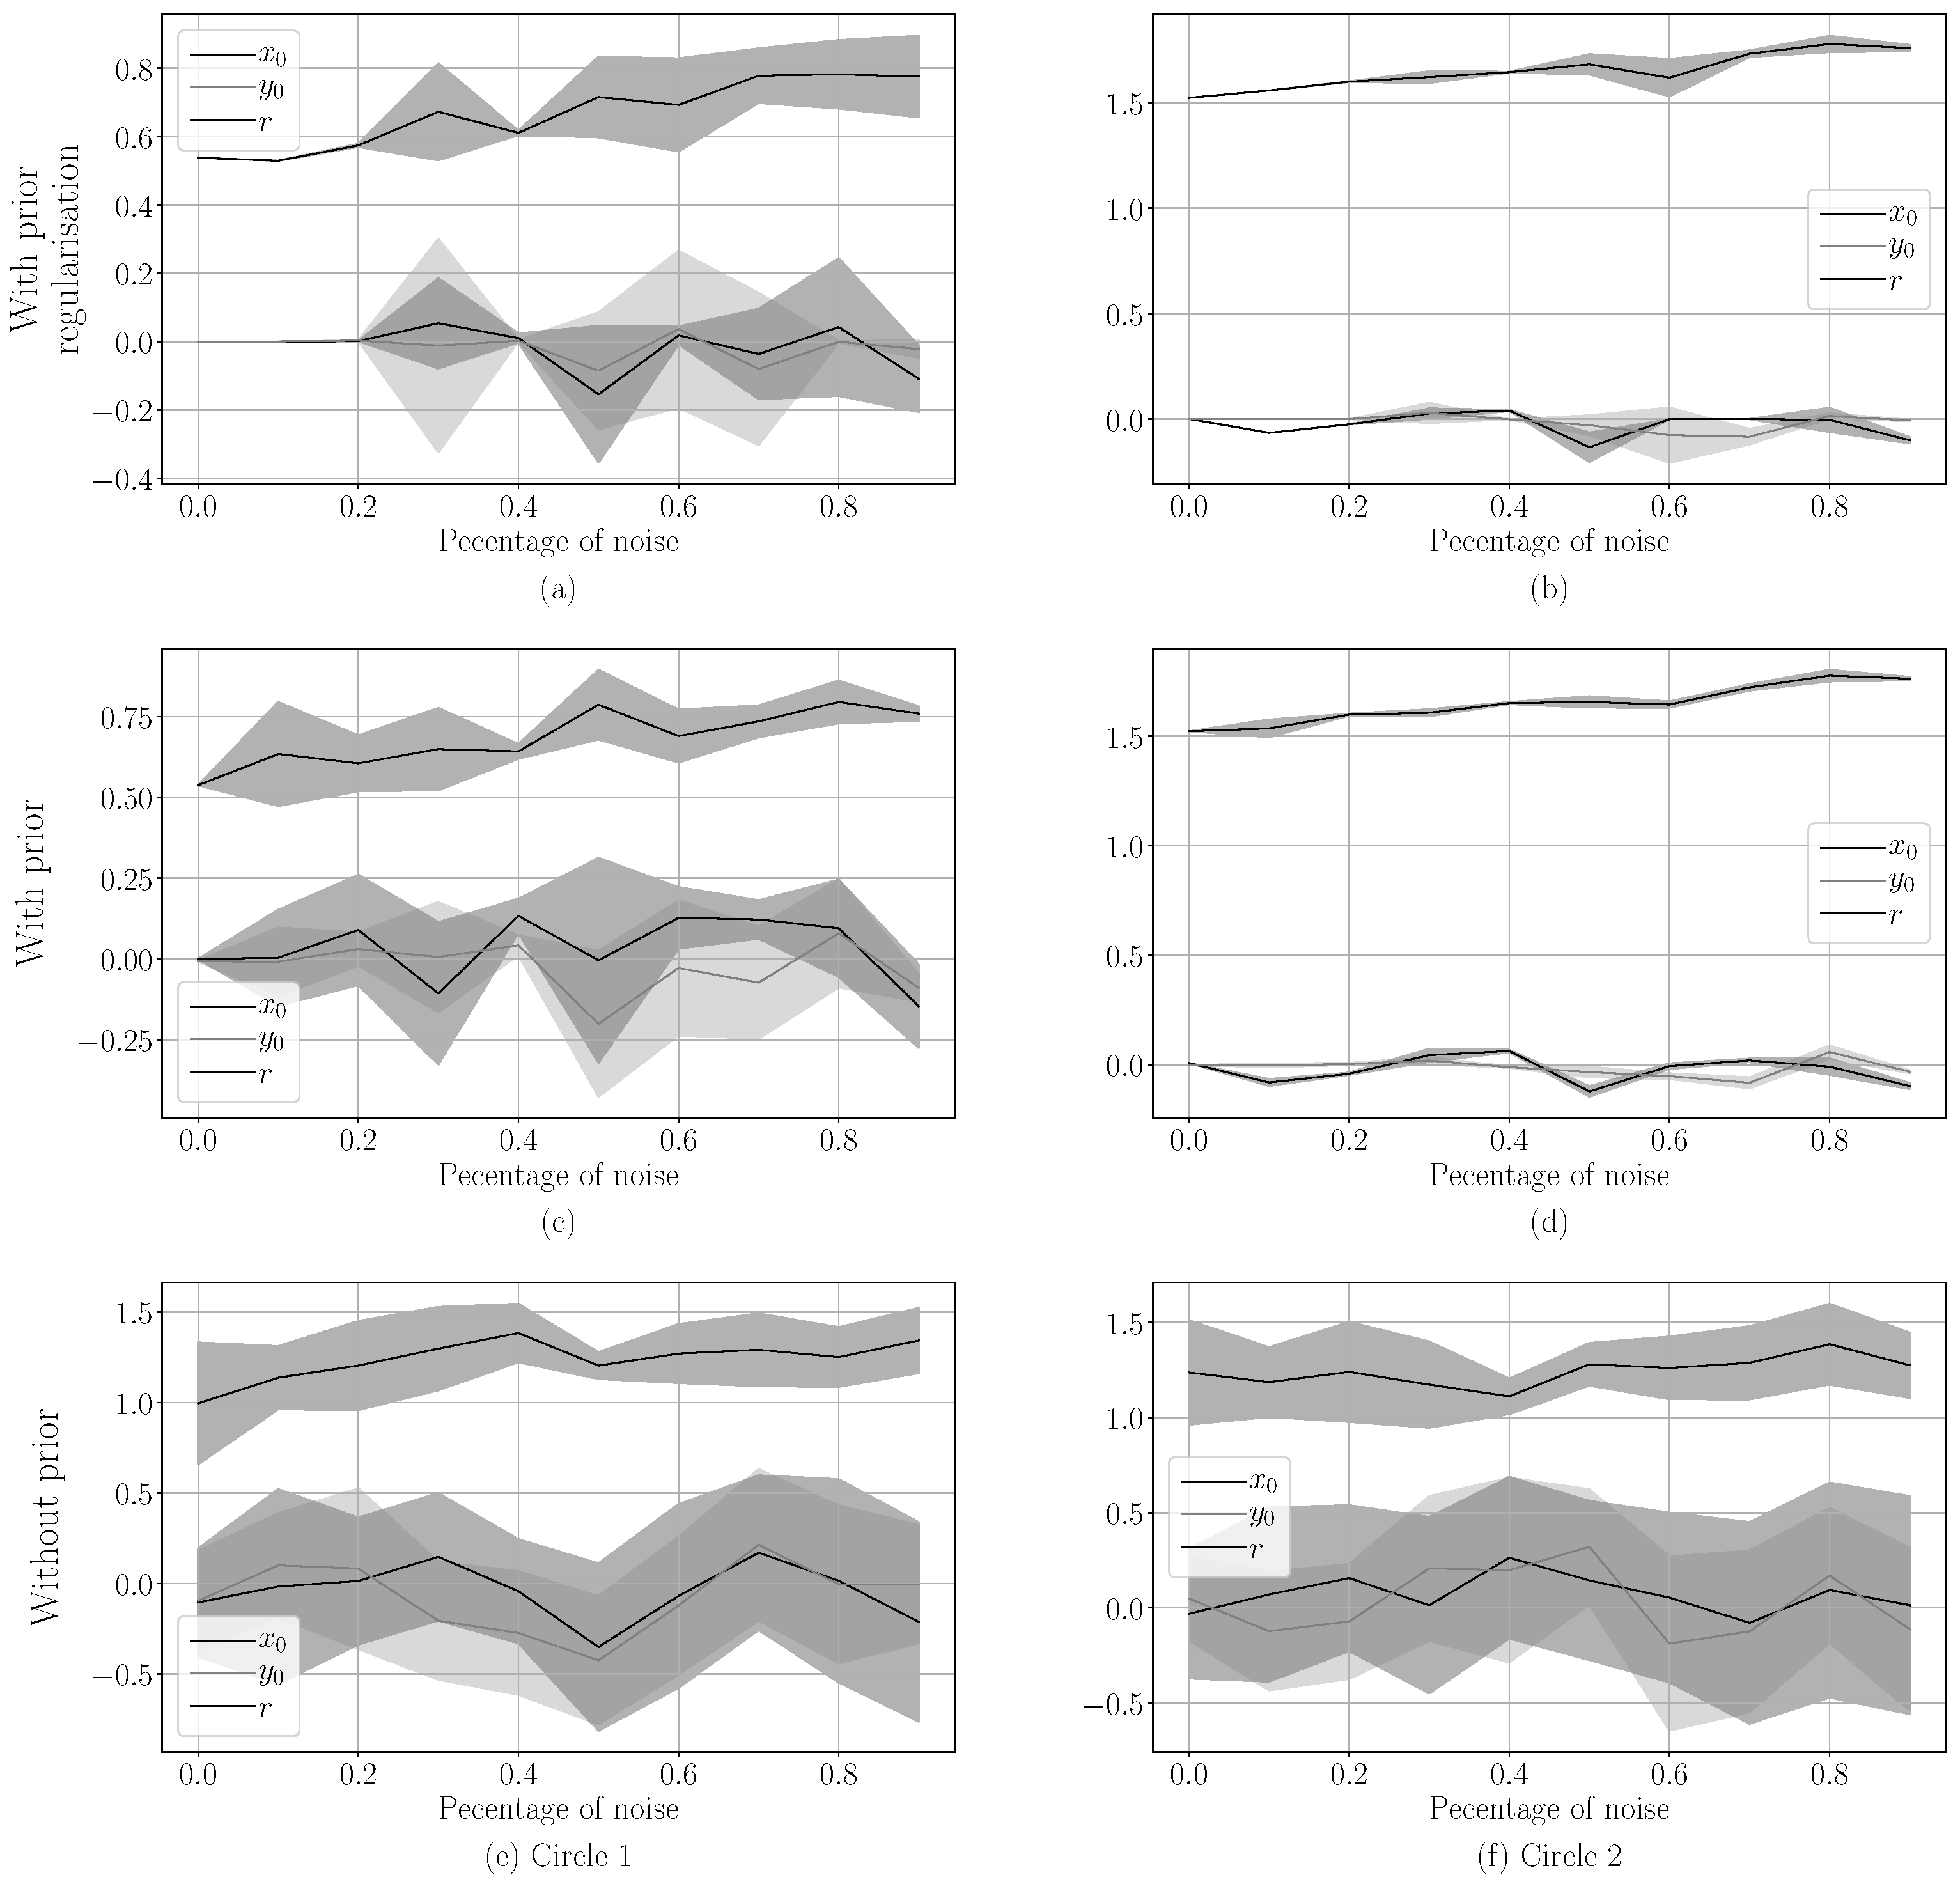
\includegraphics[width=1\textwidth]{result_eng/experiment_synthetic_param_progress_noise}
\caption{The dependence of center and radius on the noise level: (a)--(b) multimodel with prior regularization; (c)--(d) multimodel with simple prior; (e)--(f) multimodel without any priors.}
\label{experiment:st:3:1}
\end{figure}

\begin{figure}[h!t]\center
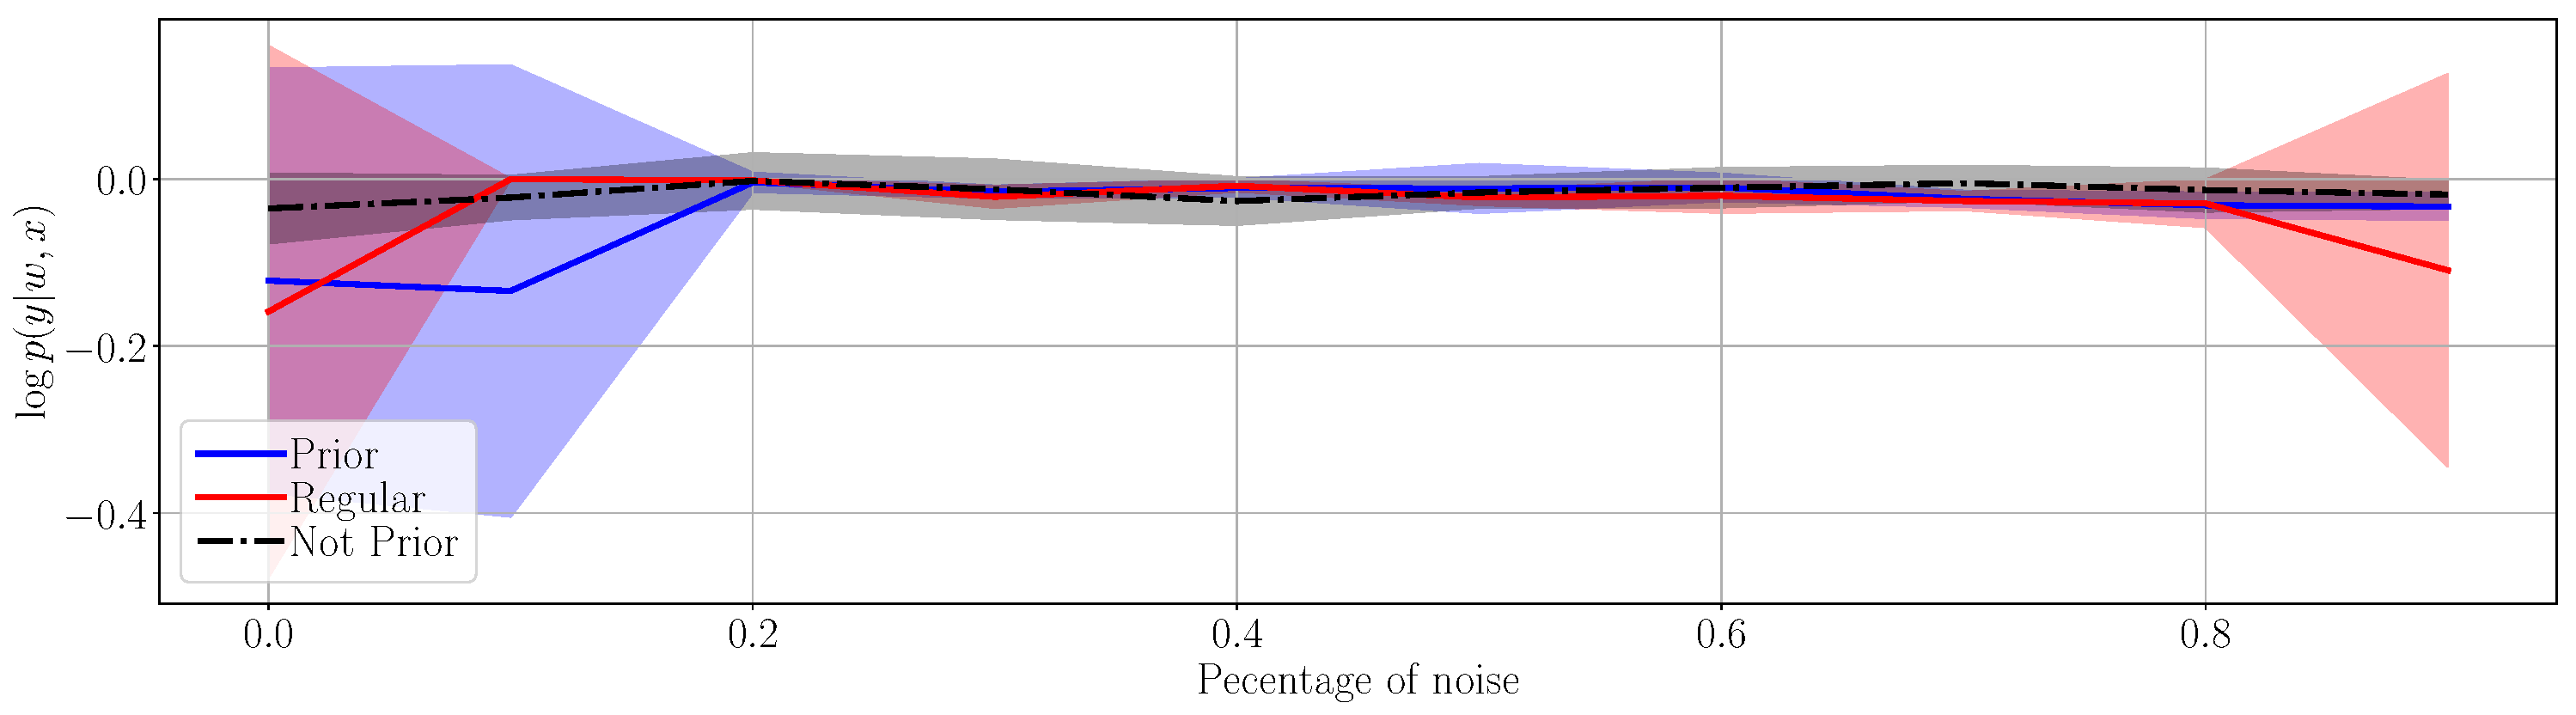
\includegraphics[width=1\textwidth]{result_eng/experiment_synt_likelihood_progress_noise}
\caption{The dependence of log-likelihood~\eqref{eq:st:new:1} on the noise level.}
\label{experiment:st:3:2}
\end{figure}

The experiment analyzes dependence of multimodels~$\textbf{f}_1, \textbf{f}_2, \textbf{f}_3$ on the noise level. 
The multimodels were analysed on the synthetic dataset~Synthetic~1, with adding various noise level.
The lowest noise level is equal to~$0$, when number of noise samples is equal to $0$. The highest noise level is equal to~$1$, when number of noise samples is equal to number of point in circles.
Fig.~\ref{experiment:st:3:1} shows the dependence of center and radius on the noise level. It shows that circle radius increases with increasing noise level. 
The multimodels~$\textbf{f}_2, \textbf{f}_3$ approximate circles center correctly, but the multimodel~$ \textbf{f}_3$ is more stable.
Fig.~\ref{experiment:st:3:2} shows the dependence of log-likelihood~\eqref{eq:st:new:1} on the noise level. 
It shows that log-likelihood~\eqref{eq:st:new:1} is the same for all multimodels, but the fig.~\ref{experiment:st:3:1} shows that the approximation quality~\eqref{eq:ce:ex:0:1} depends on multimodels.
This part of the experiment shows that multimodel~$\textbf{f}_3$ with prior regularisation is the most stable model.

\paragraph{Real data.}
\begin{figure}[h!t]\center
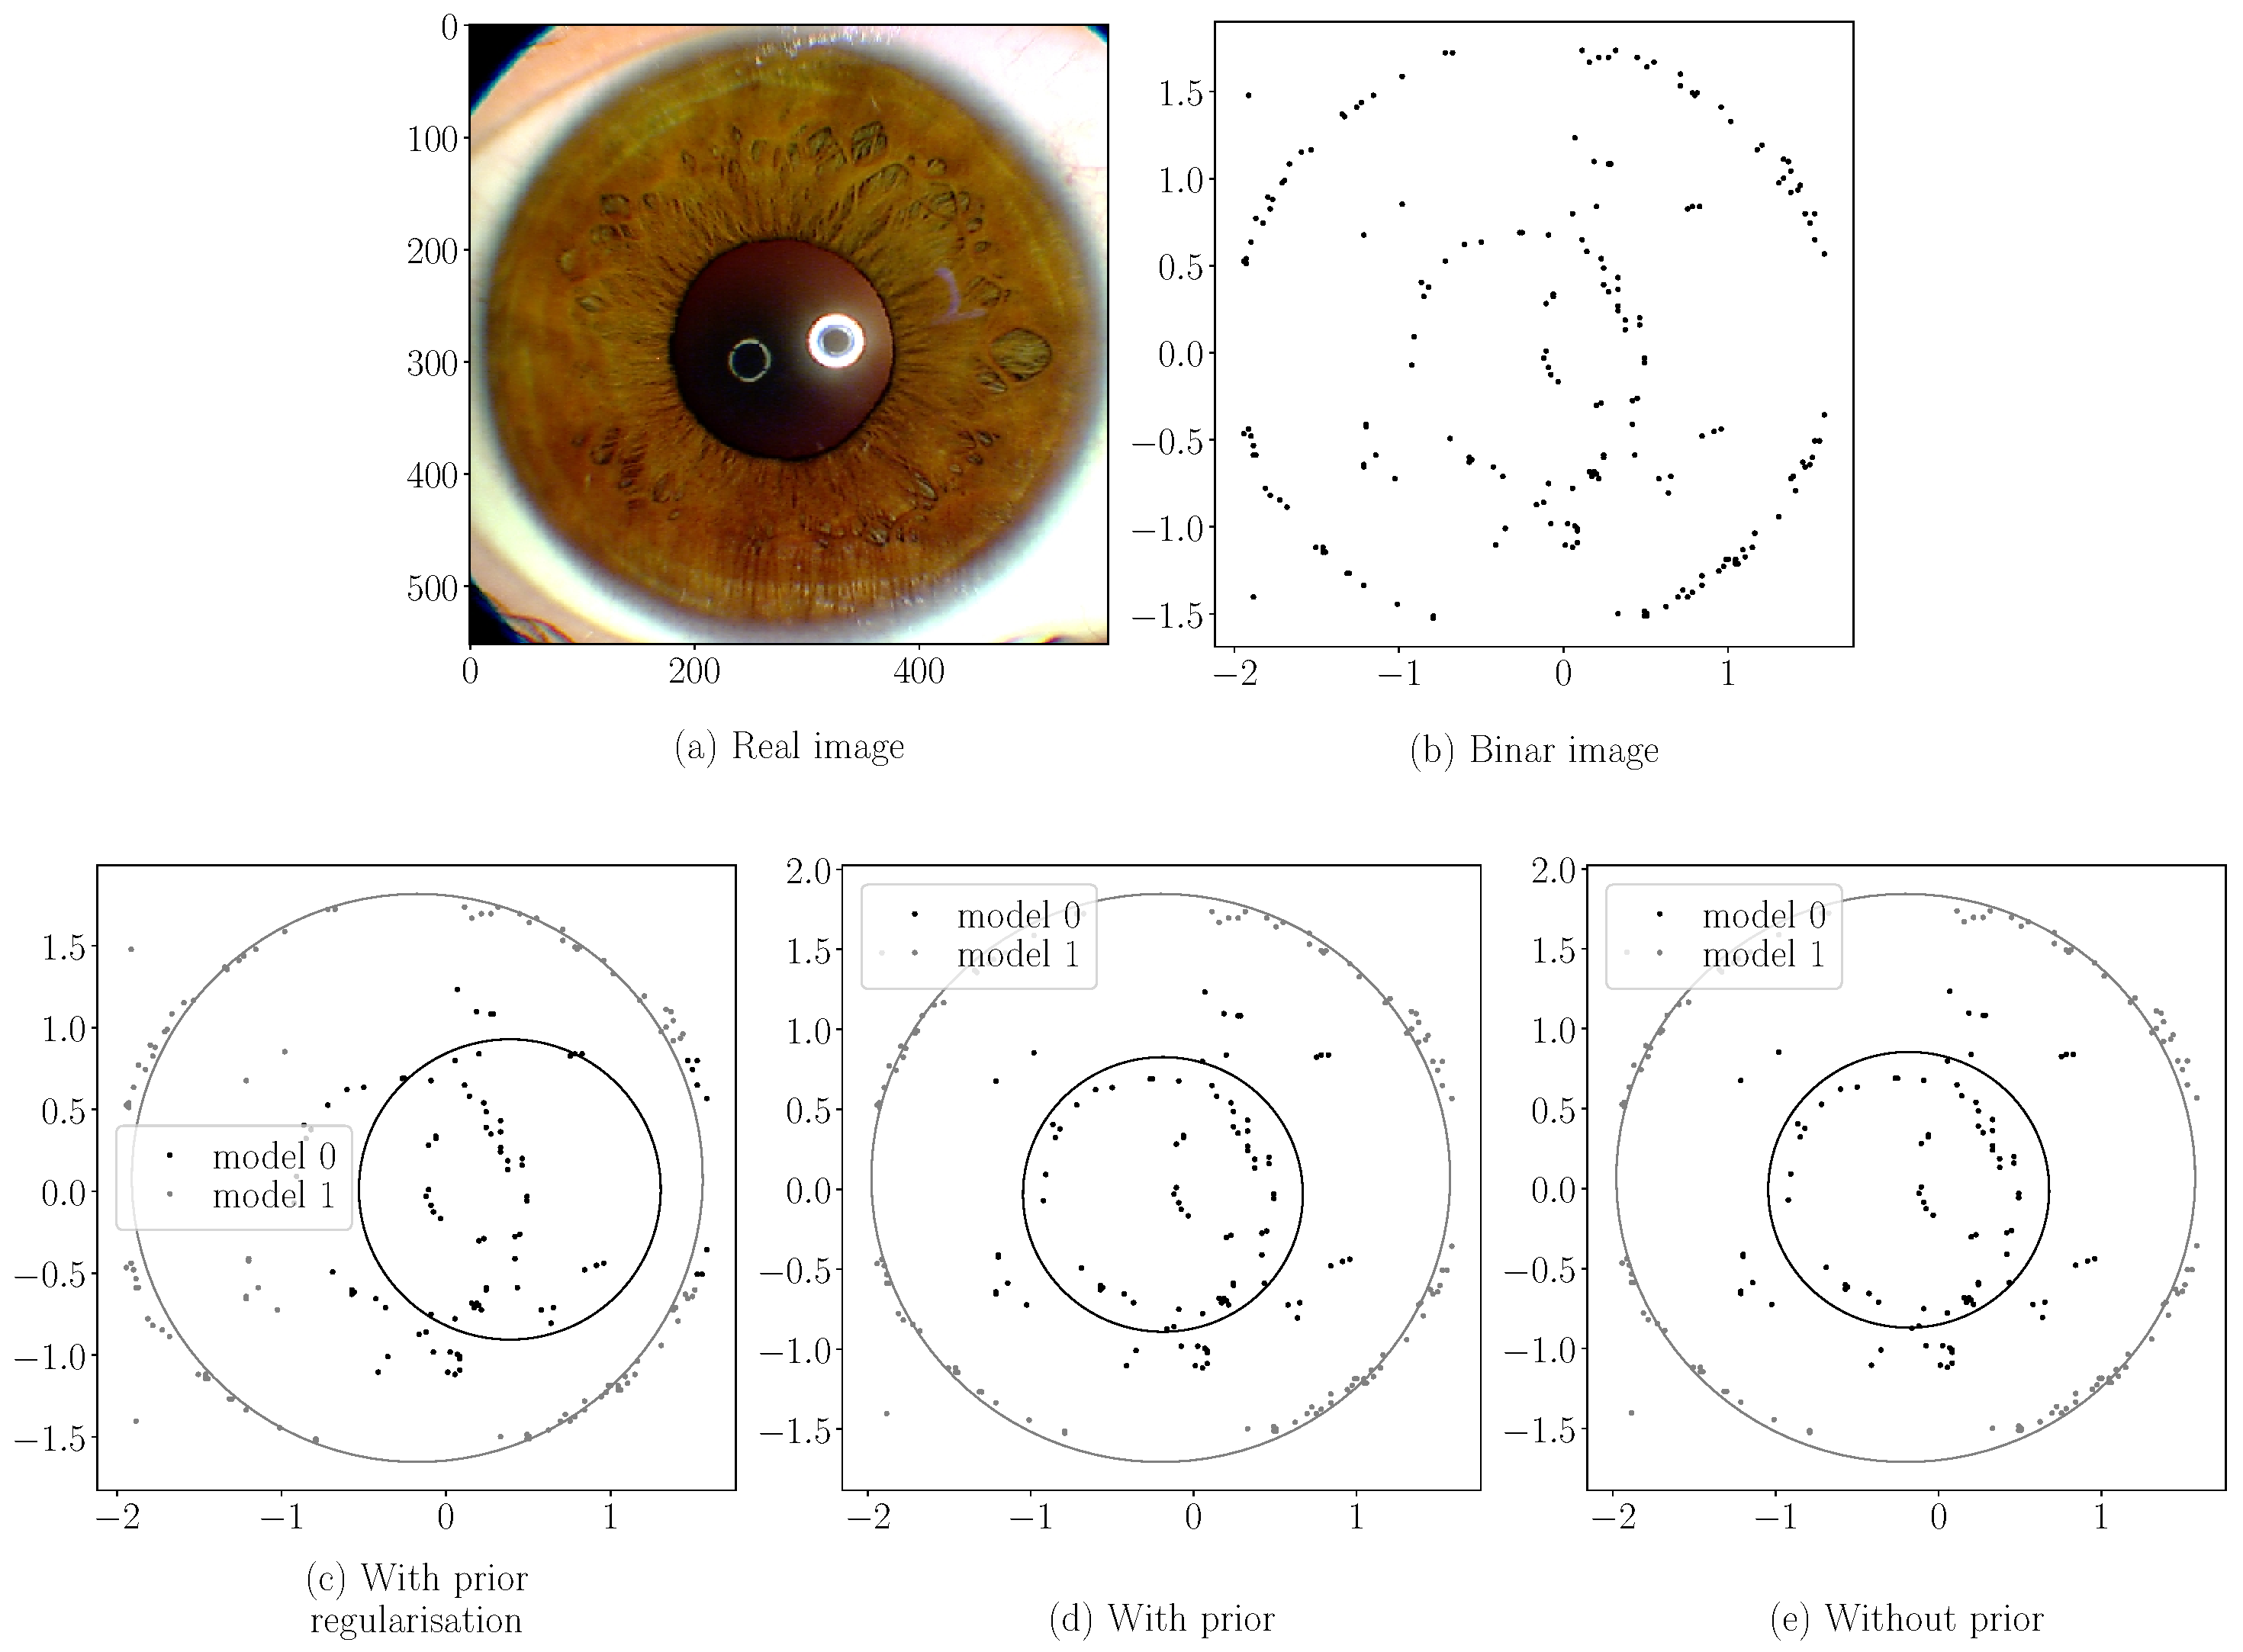
\includegraphics[width=0.9\textwidth]{result_eng/experiment_real_compare}
\caption{Different multimodels on the real image: (a) source image; (b) binarize image; (c) multimodel without any priors; (d) multimodel with simple prior; (e) multimodel with prior regularisation.}
\label{experiment:2}
\end{figure}

This part of the experiment analyzes multimodels~$\textbf{f}_1, \textbf{f}_2, \textbf{f}_3$ on the real data.
Fig.~\ref{experiment:2} shows the result of different multimodels.
The multimodel~$\textbf{f}_1$ approximates incorrectly one of the circles.
The multimodels~$\textbf{f}_2, \textbf{f}_3$ approximate both circles correctly.

\begin{figure}[h!t]\center
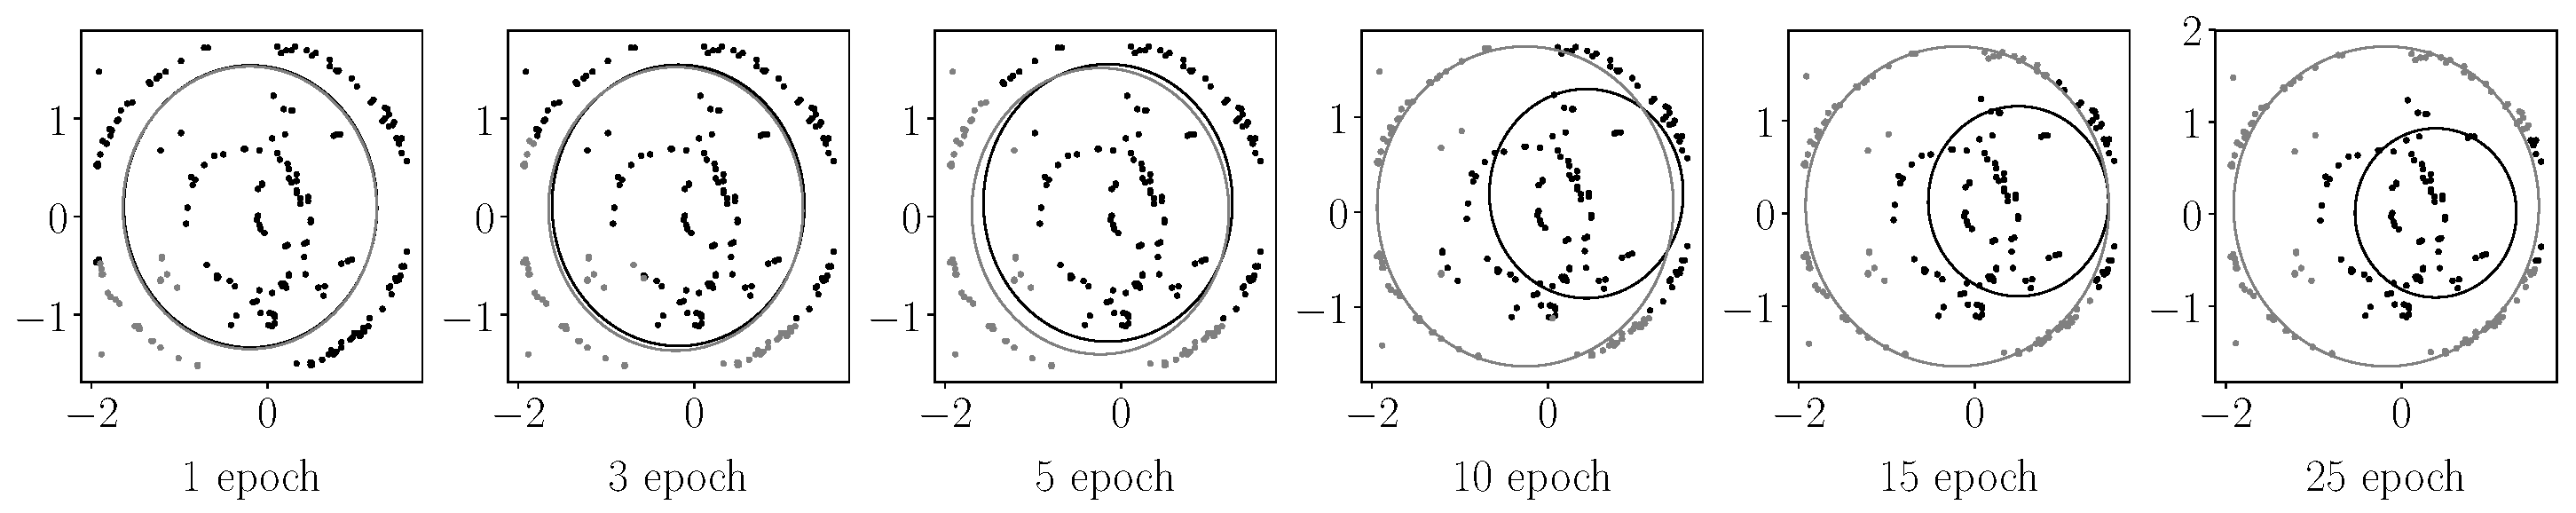
\includegraphics[width=1\textwidth]{result_eng/experiment_real_not_prior}
\caption{Visualization of convergence for the multimodel without any priors.}
\label{experiment:3}
\end{figure}

\begin{figure}[h!t]\center
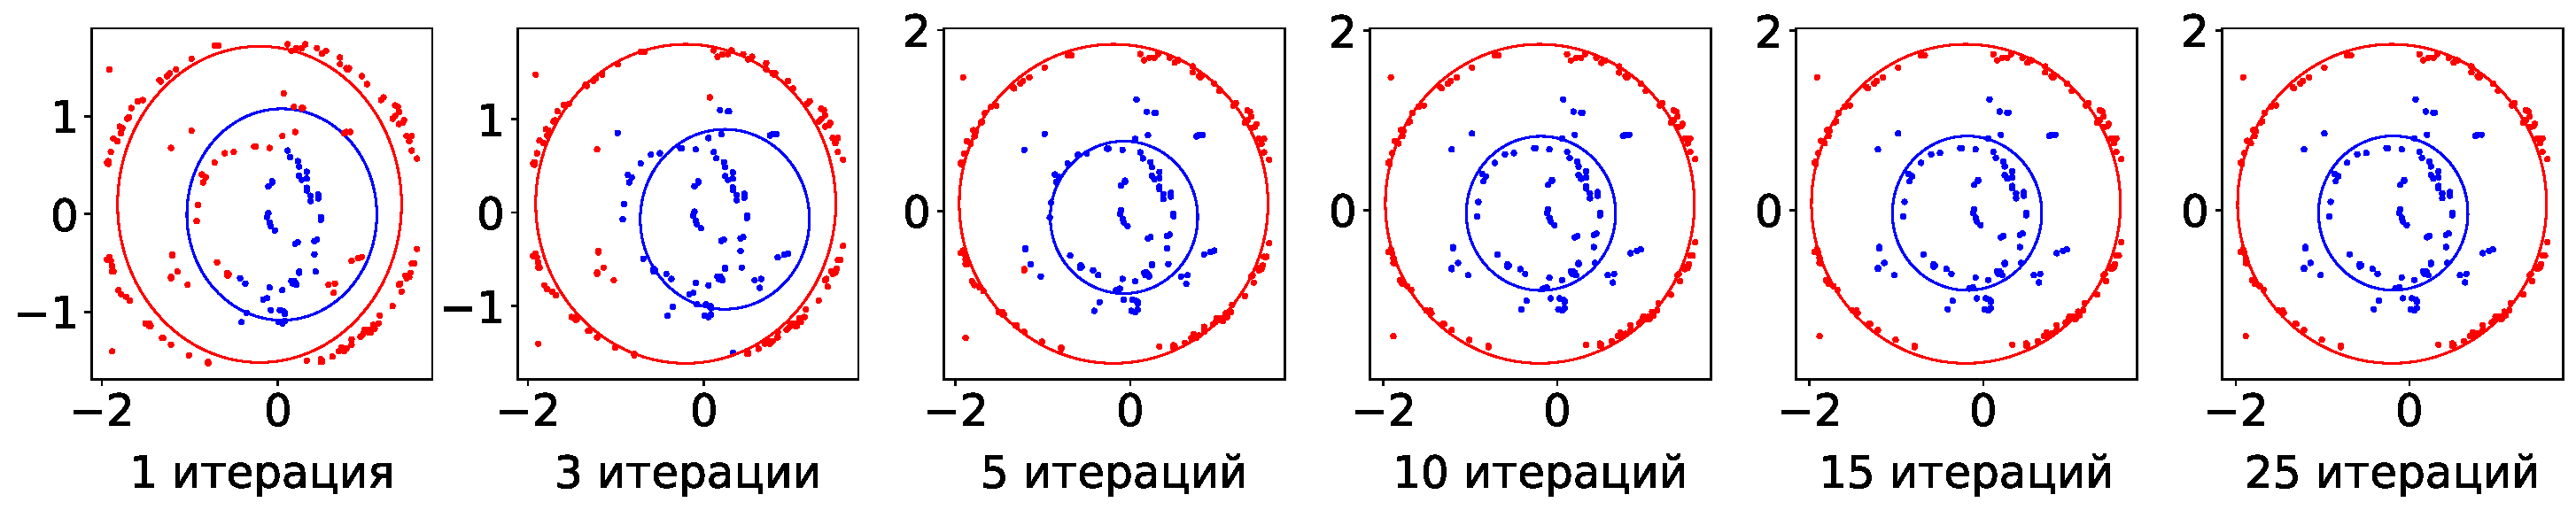
\includegraphics[width=1\textwidth]{result_eng/experiment_real_prior}
\caption{Visualization of convergence for the multimodel with simple prior.}
\label{experiment:4}
\end{figure}

\begin{figure}[h!t]\center
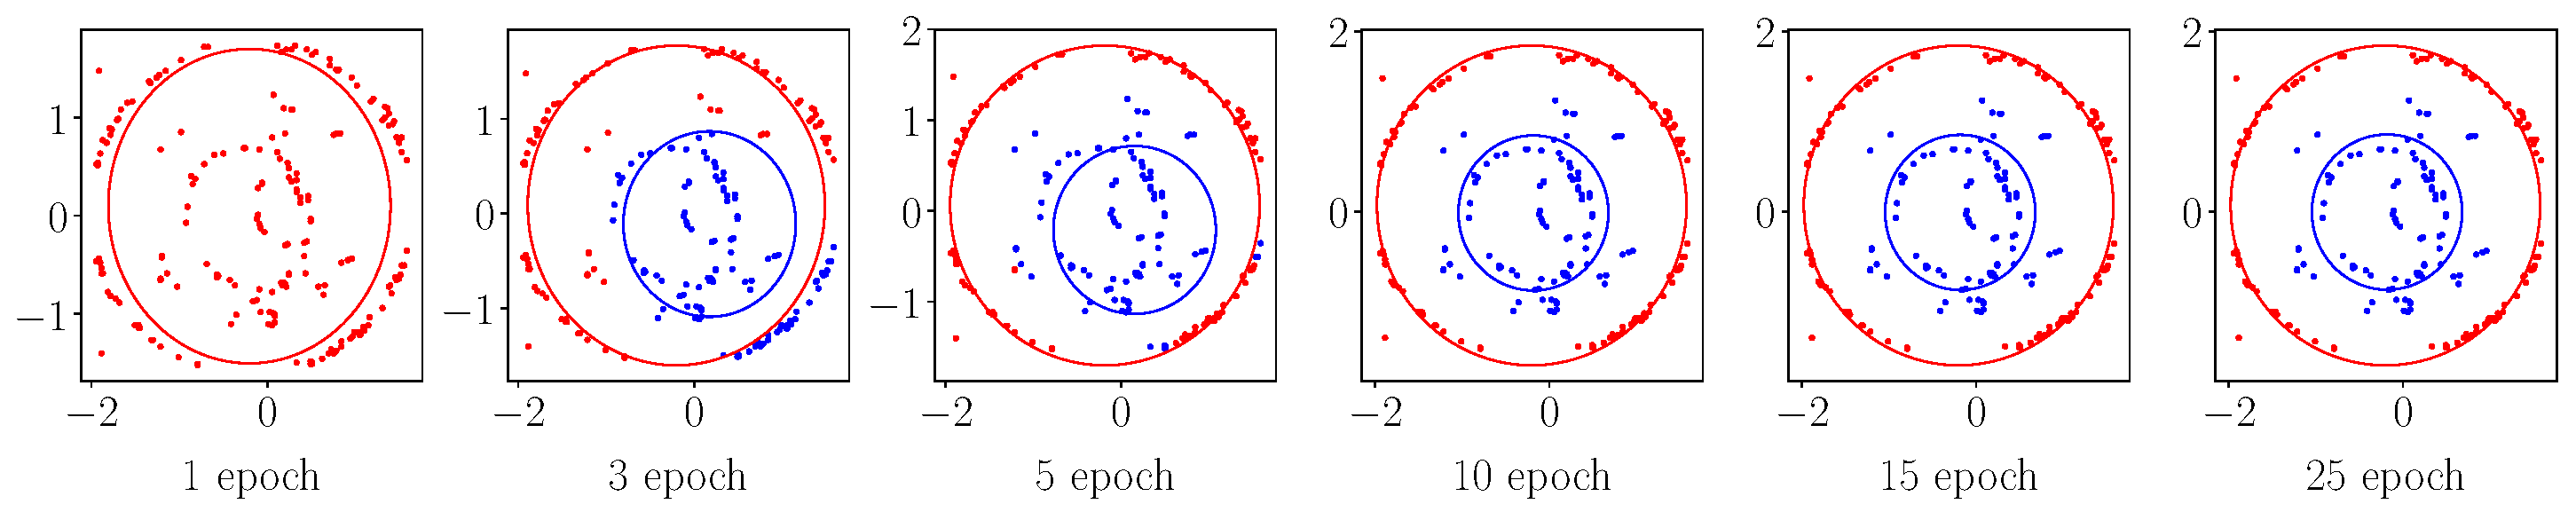
\includegraphics[width=1\textwidth]{result_eng/experiment_real_regular}
\caption{Visualization of convergence for the multimodel with prior regularisation.}
\label{experiment:5}
\end{figure}

Fig.~\ref{experiment:3}-\ref{experiment:5} show learning process for multimodels~$\textbf{f}_1, \textbf{f}_2, \textbf{f}_3$.
Fig.~\ref{experiment:3} shows multimodel~$\textbf{f}_1$.
Fig.~\ref{experiment:4} shows multimodel~$\textbf{f}_2$.
Fig.~\ref{experiment:5} shows multimodel~$\textbf{f}_3$.

This part of experiment shows that multimodels~$\textbf{f}_2, \textbf{f}_3$ approximate circles better than multimodel~$\textbf{f}_1$ even for the real images.


\section{Conclusion}
The paper compares multimodels with various prior distributions of model parameters. 
The computational experiment hold on the concentric circles with different noises.
The linear models were used to approximate the circles in the image. The gate function is the two-layer fully connected neural network.
The experiment compares the multimodel with the prior distribution and without it. The multimodel with prior distribution is more accurate in comparison to the multimodel without it.
Another experiment compares different types of regularization. The experiment showed that multimodel with regularization is more stable.
The experiment shows that all models in this article are sensitive to outlines. To solve this problem, the aouthors proposed to use a local model, which approximate noise. 

The future work plannes to improve the multimodel by adding a prior distribution for the gate function parameters. It plannes to add a local model that approximates noise in the data. It assumes that the probability of noise is low.

\begin{thebibliography}{99}
\bibitem{Tianqi2016}
	\textit{Tianqi~C., Carlos~G.} XGBoost: A Scalable Tree Boosting System~// Proceedings of the 22nd ACM SIGKDD International Conference on Knowledge Discovery and Data Mining. 2016.
	
\bibitem{Ishwaran2012}
	\textit{Xi~C., Hemant~I.} Random Forests for Genomic Data Analysis~// Genomics. 2012. Issues.~99. \No~6. P.~323--329.

\bibitem{Yuksel2012}
	\textit{Esen~Y.\,S., Wilson~J., Gader~P.\,D.} Twenty Years of Mixture of Experts~// IEEE Transactions on Neural Networks and Learning Systems. 2012. Issues.~23. \No~8. P.~1177--1193.

\bibitem{Edward2002}
	\textit{Rasmussen~C.\,E., Ghahramani~Z.} Infinite Mixtures of Gaussian Process Experts~// Advances in Neural Information Processing Systems 14. 2002. P.~881--888.

\bibitem{Shazeer2017}
	\textit{Shazeer~N., Mirhoseini~A., Maziarz~K.} Outrageously large neural networks: the sparsely-gated mixture-of-experts layer~//  International Conference on Learning Representations. 2017.
	
\bibitem{Jordan1994}
	\textit{Jordan~M.\,I.} Hierarchical mixtures of experts and the EM algorithm~// Neural Comput. 1994. Vol.~6, \No~2. P.~181--214.
	
\bibitem{Jordan1991}
	\textit{Jordan~M.\,I., Jacobs~R.\,A.} Hierarchies of adaptive experts~// In Advances in Neural Information Processing Systems. 1991. P.~985--992.
	
\bibitem{Lima2007}
	\textit{Lima~C., Coelho~A., Zuben~F.\,J.} Hybridizing mixtures of experts with support vector machines: Investigation into nonlinear dynamic systems identification~// Inf. Sci. 2007. Vol.~177. \No~10. P.~2049--2074.

\bibitem{Cao2003}
	\textit{Cao~L.} Support vector machines experts for time series forecasting~// Neurocomputing. 2003. Vol.~51. P.~321--339.
	
\bibitem{Yumlu2003}
	\textit{Yumlu~M.\,S., Gurgen~F.\,S.,  Okay~N.} Financial time series prediction using mixture of experts~// In Proc. 18th Int. Symp. Comput. Inf. Sci. 2003. P.~553--560.
	
\bibitem{Cheung1995}
	\textit{Cheung~Y.\,M., Leung~W.\,M., Xu~L.} Application of mixture of experts model to financial time series forecasting~// On Proc. Int. Conf. Neural Netw. Signal Process. 1995. P.~1--4.
	
\bibitem{Weigend2000}
	\textit{Weigend~A.\,S., Shi~S.} Predicting daily probability distributions of S\&P500 returns~// J. Forecast. 2000. Vol.~19. \No~4. P.~375--392.
	
\bibitem{Ebrahimpour2009}
	\textit{Ebrahimpour~R., Moradian~M.\,R., Esmkhani~A., Jafarlou~F.\,M.} Recognition of Persian handwritten digits using characterization loci and mixture of experts~// J. Digital Content Technol. Appl. 2009. Vol.~3. \No~3. P.~42--46.
	
\bibitem{Estabrooks2001}
	\textit{Estabrooks~A., Japkowicz~N.} A mixture-of-experts framework for text classification~//In Proc. Workshop Comput. Natural Lang. Learn., Assoc. Comput. Linguist. 2001. P.~1--8.
	
\bibitem{Mossavat2010}
	\textit{Mossavat~S., Amft~O., Petkov~Vries~B., Kleijn~W.} A Bayesian hierarchical mixture of experts approach to estimate speech quality~// In Proc. 2nd Int. Workshop Qual. Multimedia Exper. 2010. P.~200--205. 

\bibitem{Peng1996}
	\textit{Peng~F., Jacobs~R.\,A., Tanner~M.\,A.} Bayesian inference in mixtures-of-experts and hierarchical mixtures-of-experts models with an application to speech recognition~// J. Amer. Stat. Assoc. 1996. Vol.~91. \No~435. P. 953--960.
	
\bibitem{Tuerk2001}
	\textit{Tuerk~A.} The state based mixture of experts HMM with applications to the recognition of spontaneous speech. Ph.D. thesis. Cambridge: Univ. Cambridge, 2001.
	
\bibitem{Sminchisescu2007}
	\textit{Sminchisescu~C., Kanaujia~A., Metaxas~D.} Discriminative density propagation for visual tracking~// IEEE Trans. Pattern Anal. Mach. Intell. 2007. Vol.~29. \No~11. P. 2030--2044.

\bibitem{Bowyer2010}
	\textit{Bowyer~K., Hollingsworth~K., Flynn~P.} A Survey of Iris Biometrics Research: 2008--2010.
	
\bibitem{Matveev2010}
	\textit{Matveev~I.} Detection of iris in image by interrelated maxima of brightness gradient projections~// Appl.Comput. Math. 2010. Vol.~9. \No~2. P. 252--257.

\bibitem{Matveev2014}
	\textit{Matveev~I., Simonenko~I.}. Detecting precise iris boundaries by circular shortest path method~// Pattern Recognition and Image Analysis. 2014. Vol. 24. P. 304--309.
	
\bibitem{Dempster1977}
	\textit{Dempster~A.\,P., Laird~N.\,M., Rubin~D.\,B.} Maximum Likelihood from Incomplete Data via the EM Algorithm~// Journal of the Royal Statistical Society. Series B (Methodological). 1977. Vol. 39. \No~1 P. 1--38.
	
\bibitem{bishop2006}
	\textit{Bishop~C.} Pattern Recognition and Machine Learning. Berlin: Springer, 2006. P. 758.

 \end{thebibliography}


\end{document}

